% \iffalse meta-comment
%<=*COPYRIGHT>
%% Copyright (C) 2011-2012 by Martin Scharrer <martin@scharrer-online.de>
%% ----------------------------------------------------------------------
%% This work may be distributed and/or modified under the
%% conditions of the LaTeX Project Public License, either version 1.3
%% of this license or (at your option) any later version.
%% The latest version of this license is in
%%   http://www.latex-project.org/lppl.txt
%% and version 1.3 or later is part of all distributions of LaTeX
%% version 2005/12/01 or later.
%%
%% This work has the LPPL maintenance status `maintained'.
%%
%% The Current Maintainer of this work is Martin Scharrer.
%%
%% This work consists of the files trimclip.dtx, adjustbox.ins
%% and the derived files trimclip.sty,
%% tc-dvips.def, tc-pdftex.def, tc-pgf.def and tc-xetex.def.
%% Further author information are located in the .def files.
%%
%<=/COPYRIGHT>
% \fi
%
% \iffalse
%<*driver>
\ProvidesFile{trimclip.dtx}[%
%<=*DATE>
    2012/05/16
%<=/DATE>
%<=*VERSION>
    v1.0
%<=/VERSION>
    DTX file for the trimclip package]
\documentclass[a4paper]{ydoc}[2011/11/16]
\GetFileInfo{trimclip.dtx}
\usepackage{trimclip}[\filedate]

\usepackage[utf8]{inputenc}
\usepackage{standalone}

%\AtBeginDocument{\MakeShortMacroArgs\`\relax}
%\AtEndDocument{\DeleteShortVerb\`}
%
\normalmarginpar

\usepackage{flafter}

\usepackage{tikz}
\usetikzlibrary{calc}
\newsavebox\mybox

\renewenvironment{example}[1][Example:]{%
    \subsubsection*{#1}%
}{%
    \par
}
\newenvironment{examples}[1][Examples:]{%
    \subsubsection*{#1}%
}{%
    \par
}
\optionaloff

\lstdefinelanguage{none}{}%
\lstdefinelanguage{adjustbox}{%
  moretexcs={%
      begin,end,adjustbox
  },
  emph={%
      frame,fbox,cframe,cfbox,minipage,raise
  },
}%

\lstdefinestyle{examplecode}{%
    basicstyle=\ttfamily\small,
    numbers=none,language=none,
    classoffset=1,
    morekeywords={begin,end},
    keywordstyle=\bfseries,
    classoffset=0,
    morekeywords={adjustbox,minsizebox,maxsizebox,lapbox,marginbox,phantombox},
    keywordstyle=\macrodescstyle,
}

\makeatletter
\def\PrintExample{%
  \begingroup
  \par\smallskip\noindent
  \leavevmode
  \BoxExample
  \@tempdima=\textwidth
  \advance\@tempdima by -\wd\examplecodebox\relax
  \advance\@tempdima by -\wd\exampleresultbox\relax
  \advance\@tempdima by -15pt\relax
  \ifdim\@tempdima>\bigskipamount
    \hbox to \textwidth{%
     \null\hss
     \minipage[c]{\wd\examplecodebox}\usebox\examplecodebox\endminipage
     \hfill\hskip\bigskipamount\hfill
     \minipage[c]{\wd\exampleresultbox}%
        \EXAMPLERESULT
     \endminipage
     \hss\null
     }%
  \else
    \vbox{%
        \leftline{\usebox\examplecodebox}%
        \vspace{\bigskipamount}%
        \rightline{\EXAMPLERESULT}%
    }%
  \fi
  \par\smallskip
  \endgroup
}
\def\EXAMPLERESULT{%
    \leavevmode\hbox{%
    \textcolor{exampleborder}{%
        \boxframe
            {\dimexpr\wd\exampleresultbox+2\fboxrule\relax}%
            {\dimexpr\ht\exampleresultbox+\fboxrule\relax}%
            {\dimexpr\dp\exampleresultbox+\fboxrule\relax}%
        \hskip-\wd\exampleresultbox
        \hskip-\fboxrule
        \rule[-.25\fboxrule]{\wd\exampleresultbox}{.5\fboxrule}%
        \hskip-\wd\exampleresultbox
    }%
    \usebox\exampleresultbox
    }%
}%
\makeatother
\colorlet{exampleborder}{black!33}
\def\Descsep{\par\vskip-2.5ex\relax}

\def\examplecontent{\raisebox{-4pt}{\begin{tabular}[b]{@{}|c|c|@{}}
      \hline
      A & B \\
      \hline
      C & D \\
      \hline
  \end{tabular}%
}}

%\EnableCrossrefs
%\CodelineIndex
%\RecordChanges
\OnlyDescription
\renewcommand\topfraction{.9}
\renewcommand\bottomfraction{.9}
\renewcommand\textfraction{.1}
\renewcommand\floatpagefraction{.5}
\renewcommand\dbltopfraction{.7}
\renewcommand\dblfloatpagefraction{.5}
\begin{document}
 \DocInput{trimclip.dtx}
  \PrintChanges
  %\newpage\PrintIndex
\end{document}
%</driver>
% \fi
%
% \CheckSum{490}
%
% \CharacterTable
%  {Upper-case    \A\B\C\D\E\F\G\H\I\J\K\L\M\N\O\P\Q\R\S\T\U\V\W\X\Y\Z
%   Lower-case    \a\b\c\d\e\f\g\h\i\j\k\l\m\n\o\p\q\r\s\t\u\v\w\x\y\z
%   Digits        \0\1\2\3\4\5\6\7\8\9
%   Exclamation   \!     Double quote  \"     Hash (number) \#
%   Dollar        \$     Percent       \%     Ampersand     \&
%   Acute accent  \'     Left paren    \(     Right paren   \)
%   Asterisk      \*     Plus          \+     Comma         \,
%   Minus         \-     Point         \.     Solidus       \/
%   Colon         \:     Semicolon     \;     Less than     \<
%   Equals        \=     Greater than  \>     Question mark \?
%   Commercial at \@     Left bracket  \[     Backslash     \\
%   Right bracket \]     Circumflex    \^     Underscore    \_
%   Grave accent  \`     Left brace    \{     Vertical bar  \|
%   Right brace   \}     Tilde         \~}
%
%
% \changes{v1.0}{2012/05/16}{First version after extraction from \pkg{adjustbox} package.}
%
% \GetFileInfo{trimclip.dtx}
%
% \DoNotIndex{\newcommand,\newenvironment,\def,\edef,\xdef,\gdef,\let}
% \bundle{adjustbox}
% \author{Martin Scharrer}
% \email{martin@scharrer-online.de}
% ^^A\repository{https://bitbucket.org/martin_scharrer/adjustbox}
% \ydocpdfsettings
% \maketitle
%
% \makeatletter
% \def\LATeX{\texorpdfstring{(L\kern -.36em{\sbox \z@ T\vbox to\ht \z@ {\hbox {\check@mathfonts
%  \fontsize \sf@size \z@ \math@fontsfalse \selectfont A}\vss }}\kern -.15em)\TeX}{(La)TeX}}
% \makeatother
%
% \vspace{-\baselineskip}
% \begin{abstract}
% This package extends the standard \pkg{graphicx} package by providing the missing \Macro\trimbox and \Macro\clipbox
% macros to trim and clip arbitrary \TeX\ material.
% The macros allow for verbatim content. Equivalent environments are also provided.
% The package comes with own clipping drivers for all common output formats as well as a \pkg{pgf} fall-back driver.
% \end{abstract}
%
% \section{Introduction}
% The standard \LaTeX{} package \pkg{graphicx}.^^A\footnote{Actually it is the \pkg{graphics} package, but
% ^^Athis is assumed to be completely superseded by its extension \pkg{graphicx}.}
% allows to scale, resize and rotate either images or text (i.e.\ any \TeX\ content).  For text the macros
% \Macro\scalebox, \Macro\resizebox and \Macro\rotatebox can be used, while equivalent keys exist for the
% \Macro\includegraphics macro.  However, while it is possible to trim and clip images using the \Key{trim}, \Key{viewport}
% and \Key{clip} keys, no equivalent macros are provided.  This package closes this gap by defining the macros
% \Macro\trimbox and \Macro\clipbox. As an extra the macro \Macro\marginbox is also provided.  It can be seen as an
% inverted \Macro\trimbox, expanding the official size of the content instead of reducing it.
% Originally these macros were included in the \pkg{adjustbox} package together with the general \Macro\adjustbox macro.
% However, the fundamental clip and trim macros and their driver files are now packed into this minimalistic package,
% so that other packages can reuse its functionality without the need to load the ever-growing \pkg{adjustbox} package.
%
% \enlargethispage{\baselineskip}
% The macros provided by this package differ in three aspects from the macros defined by \pkg{graphicx}.  The content
% argument is actually read directly as a horizontal box and not as a macro argument, even when the syntax looks the
% same.  This allows for arbitrary content including special things like verbatim material. It is allowed to replace the
% "{ }" around the content with \Macro\bgroup and \Macro\egroup.  Furthermore, for every macro there is an equivalent
% environment with the same name. Special care is taken to allow the same name for both, which is normally not allowed.
% Finally, the lengths arguments of the macros can contain algebraic expressions to calculate the used length. This is
% only possible with the \pkg{graphicx} macros if the \pkg{calc} package is loaded. However, the \pkg{trimclip} macros
% use the \pkg{adjcalc} wrapper package which either uses $\epsilon$-\TeX\ primitives, \pkg{calc} or \pkg{pgfmath} to
% provide this feature.
%
%
% \section{Dependencies}
% This package uses the author's other packages \pkg{collectbox} (to collect the content as a real box) and
% \pkg{adjcalc} (to allow for math expressions for lengths).  The latter is part of the same \pkg{adjustbox} bundle and
% should have be installed together with \pkg{trimclip}.
%
% \section{Drivers}
% The clip operation can not be implemented using general \TeX\ commands, but is rather output format specific.  The
% clipped material is actually included unclipped and the output file (i.e.\ PDF or PS file) contains format specific
% instructions, so that the document viewer will clip the content when the document is displayed.  Depending on the used
% compilation work-flow (like |pdflatex|, |latex|+|dvips| or |latex|+|dvipdfm|, etc.) this clipping instructions must be
% passed in a different way. In order to support all of these, dedicated driver files are provided which hold the
% specific low-level instructions.  This requirement should also be known to most users from the \pkg{graphics/x},
% \pkg{(x)color} or \pkg{hyperref} packages which also require output format specific low-level instructions to
% implement their features.
%
% A set of driver files for the most common used \LaTeX\ compilers is provided with this package (see
% \autoref{sec:options} for a list).  If no suitable driver file is found, the \pkg{pgf} package is used instead to
% implement the clip operation.  This (large) package comes with its own set of driver files and should cover any other
% \LaTeX\ compilers. The \pkg{trimclip} drivers were inspired by the \pkg{graphic/x} and \pkg{pgf} driver code and
% were written by Joseph Wright of the \LaTeX3 project and Martin Scharrer (the author of this package).
%
% \section{Package Options}\label{sec:options}
% Normally the package should be loaded without any options. A suitable driver will then automatically be selected.
% However, the package accepts the following options to select the used driver manually.  Any other option is passed to the
% \pkg{graphicx} package and the driver selected by it is used.  However, this does not work if \pkg{graphicx} or
% \pkg{graphics} was already loaded before. In this case any unknown option is taken as driver and a file
% `\MacroArgs'tc-'<option>'.def'\relax' is loaded if it exits.  If not, the default PGF fall-back driver is used. PGF
% comes with a own set of drivers but is large and can be considered a significant overhead if used only for rectangular
% clipping.
%
% \begin{description}
%   \def\Option#1{\item[{{\normalfont\opt{#1}}}]}%
%   \Option{pdftex} Use the |pdftex| driver. This driver is automatically selected for |pdflatex| and |lualatex|
%                   and should not be used for any other \LaTeX\ compilers.
%   \Option{dvips} Use the |dvips| driver. This driver is automatically selected for |latex|.
%   \Option{xetex} Use the |xetex| driver. This driver is automatically selected for |xelatex|.
%   \Option{dvipdfm} Use the |xetex| driver which is also compatible with |dvipdfm|.
%   \Option{dvipdfmx} Use the |xetex| driver which is also compatible with |dvipdfmx|.
%   \Option{pgf} Use the fall-back PGF driver explicitly. This makes sense if issue with another driver are encountered.
% \end{description}
%
% It should be noted that choosing an incorrect driver will lead to clip operation not being applied (they act like trim
% operations) and may lead to a broken output file.
%
%
% \section{Argument Values}\label{sec:argval}
% All macros of this package and their matching environments require four length values which are used to change the
% left, bottom, right and top side of the content.  Because of the used \pkg{adjcalc} package complicated algebraic
% expressions can be used to calculate these amounts. The used math engine can be changed by loading \pkg{adjcalc}
% with the appropriate option before loading \pkg{trimclip}. Please see the \pkg{adjcalc} manual for more details
% on this.
% Like with the |trim| or |viewport| keys of \Macro\includegraphics the length values must be separated by spaces.
% Note that if a previous length expression ends in a macro any trailing spaces will be removed by \TeX.  Therefore it
% is required to wrap this \emph{complete} length expression in braces.
% Several examples of this are shown in the \emph{Usage} section.
% It is also possible to only provide a single length which is used for all four
% sides or only two lengths which are taken for the left/right as well as bottom/top side.  This simplifies symmetric
% operations and got inspired by Cascading Style Sheets (CSS) used to style websites.
%
% If a length value is a simple number without a unit, a default unit is substituted (usually `|bp|', \emph{big points},
% the standard PostScript and PDF unit).  This default unit can be changed using \Macro\adjcalc{'defaultunit='<unit>} or
% completely disabled (\MacroArgs'defaultunit=none'). See the \pkg{adjcalc} manual for more details.
%
% The length values can contain the following macros to refer to the original size of the content:
%
% \DescribeMacros
%    \hbox{\Macro\width~~~\Macro\height~~~\Macro\depth~~~\Macro\totalheight}%
% \endDescribeMacros
% These \LaTeX{} lengths hold the original dimensions of the content and can be used to make relative changes.  Like any
% other length registers they can be used with a factor, e.g.\ \MacroArgs'.5'\AlsoMacro\width to refer to half the
% natural width of the content.
%
%
% \section{Usage}
%
% \subsection{Trimming}
% \vspace{-\medskipamount}
% \DescribeMacro\trimbox{<llx>~<lly>~<urx>~<ury>}{<content>}
% \DescribeMacro\trimbox{<all sites>}{<content>}
% \DescribeMacro\trimbox{<left/right>~<top/bottom>}{<content>}
% \DescribeMacro\trimbox*{<llx>~<lly>~<urx>~<ury>}{<content>}
% The macro \Macro\trimbox trims the given amount from the lower left (ll) and the upper right (ur) corner of
% the box. This means that the amount \meta{llx} is trimmed from the left side, \meta{lly} from the bottom and
% \meta{urx} and \meta{ury} from the right and top of the box, respectively.
% If only one value is given it will be used for all four sites.
% If only two values are given the first one will be used for the left and right side (llx, urx) and the second for the bottom and top side (lly, ury).
%
% If the starred version is used the four coordinates are taken as the \Key{viewport} instead, i.e. the box
% is trimmed to the rectangle described by the coordinates. In this case all four values must be specified explicitly.
%
% \begin{examples}
%   \begin{examplecode}
%   \examplecontent
%   \end{examplecode}
%   \begin{examplecode}
%   \trimbox{2pt 3pt 2pt 3pt}{\examplecontent}
%   \end{examplecode}
%   \begin{examplecode}
%   \trimbox{2pt 3pt}{\examplecontent}
%   \end{examplecode}
%   \begin{examplecode}
%   \trimbox{2pt}{\examplecontent}
%   \end{examplecode}
%   \begin{examplecode}
%   \trimbox{{.5\width} {.5\totalheight} 2pt 2pt}
%       {\examplecontent}
%   \end{examplecode}
%   \medskip
%   \begin{examplecode}
%   \trimbox*{5pt 0pt 3em 2em}{\examplecontent}
%   \end{examplecode}
%   \medskip
%   \begin{examplecode}
%   \trimbox*{5pt -2pt 3em 2em}{\examplecontent}
%   \end{examplecode}
%   \medskip
%   \begin{examplecode}
%   \trimbox*{5pt 10pt 3em 2em}{\examplecontent}
%   \end{examplecode}
%   \bigskip
%   \bigskip
%   \begin{examplecode}
%   \trimbox*{5pt -3pt 3em -1pt}{\examplecontent}
%   \end{examplecode}
% \end{examples}
%
%
% \DescribeEnv[<content>]{trimbox}{<1, 2 or 4 trim values>}
% \vspace{-\baselineskip}
% \DescribeEnv[<content>]{trimbox*}{<llx>~<lly>~<urx>~<ury>}
% The \env{trimbox} and \env{trimbox*} environments do the same as the corresponding macros.
%
%
% \Needspace*{10\baselineskip}
% \subsection{Clipping}
% \vspace{-\medskipamount}
% \DescribeMacro\clipbox{<llx>~<lly>~<urx>~<ury>}{<content>}
% \DescribeMacro\clipbox{<all sites>}{<content>}
% \DescribeMacro\clipbox{<left/right>~<top/bottom>}{<content>}
% \DescribeMacro\clipbox*{<llx>~<lly>~<urx>~<ury>}{<content>}
% The \Macro\clipbox macro works like the \Macro\trimbox and trims the given amounts from the \meta{text}.
% However, in addition the trimmed material is also clipped, i.e. it is not shown in the final document.
% Note that the material will still be part of the output file but is simply not shown.
% The full content can still be exported using special tools, so using \Macro\clipbox\relax (or \Macro\includegraphics[clip,trim=...])
% to censor classified information would be a bad idea.
% The starred version will again use the given coordinates as viewport.
%
% \DescribeEnv[<content>]{clipbox}{<1, 2 or 4 trim values>}
% \vspace{-\baselineskip}
% \DescribeEnv[<content>]{clipbox*}{<llx>~<lly>~<urx>~<ury>}
% The environment versions of \Macro\clipbox and \Macro\clipbox*. The same rules as for the trimming environments apply.
%
% \begin{examples}
%   \begin{examplecode}
%   \examplecontent
%   \end{examplecode}
%   \begin{examplecode}
%   \clipbox{2pt 3pt 2pt 3pt}{\examplecontent}
%   \end{examplecode}
%   \begin{examplecode}
%   \clipbox{2pt 3pt}{\examplecontent}
%   \end{examplecode}
%   \begin{examplecode}
%   \clipbox{2pt}{\examplecontent}
%   \end{examplecode}
%   \begin{examplecode}
%   \clipbox{{.5\width} {.5\totalheight} 2pt 2pt}
%       {\examplecontent}
%   \end{examplecode}
%   \medskip
%   \begin{examplecode}
%   \clipbox*{5pt 0pt 3em 2em}{\examplecontent}
%   \end{examplecode}
%   \medskip
%   \begin{examplecode}
%   \clipbox*{5pt -2pt 3em 2em}{\examplecontent}
%   \end{examplecode}
%   \begin{examplecode}
%   \clipbox*{5pt 10pt 3em 2em}{\examplecontent}
%   \end{examplecode}
%   \begin{examplecode}
%   \clipbox*{5pt -3pt 3em -1pt}{\examplecontent}
%   \end{examplecode}
% \end{examples}
%
% \subsection{Margin}
% \vspace{-\medskipamount}
% \DescribeMacro\marginbox{<all sites>}{<content>}
% \DescribeMacro\marginbox{<left/right>~<top/bottom>}{<content>}
% \DescribeMacro\marginbox{<llx>~<lly>~<urx>~<ury>}{<content>}
% \Descsep
% \DescribeEnv[<content>]{marginbox*}{<1, 2 or 4 margin values>}
% This macro and environment can be used to add a margin (white space) around the content. It can be seen as the opposite of \Macro\trimbox.
% The original baseline of the content is preserved because \meta{lly} is added to the depth.
%
% \begin{example}
%   \begin{examplecode}
%   Before \fbox{\marginbox{1ex 2ex 3ex 4ex}{Text}} After
%   \end{examplecode}
% \end{example}
%
%
% \DescribeMacro\marginbox'*'{<all sites>}{<content>}
% \DescribeMacro\marginbox'*'{<left/right>~<top/bottom>}{<content>}
% \DescribeMacro\marginbox'*'{<llx>~<lly>~<urx>~<ury>}{<content>}
% \Descsep
% \DescribeEnv[<content>]{marginbox}{<1, 2 or 4 margin values>}
% This starred version is almost identical to the normal \Macro\marginbox, but also raises the content by the \MacroArgs<lly>
% amount, so that the original depth is preserved instead of the original baseline.
% Note that while \Macro\marginbox is basically the opposite of \Macro\trimbox, \Macro\marginbox* is not the opposite of \Macro\trimbox*.
%
% \begin{example}
%   \begin{examplecode}
%   Before \fbox{\marginbox*{1ex 2ex 3ex 4ex}{Text}} After
%   \end{examplecode}
% \end{example}
%
%
% \clearpage
% \section{Diagrams}
% ^^A This section explains the details about the trim and clip implementations.
% ^^A It should give the interested reader a deeper understanding of the operations and the behaviour in normal and edge cases.
% The box dimensions, trim values and change of the baseline for different scenarios are visualized by the following diagrams.
%
% \begin{figure}[!bt]
%   \centering
%   {\catcode`\%=14\relax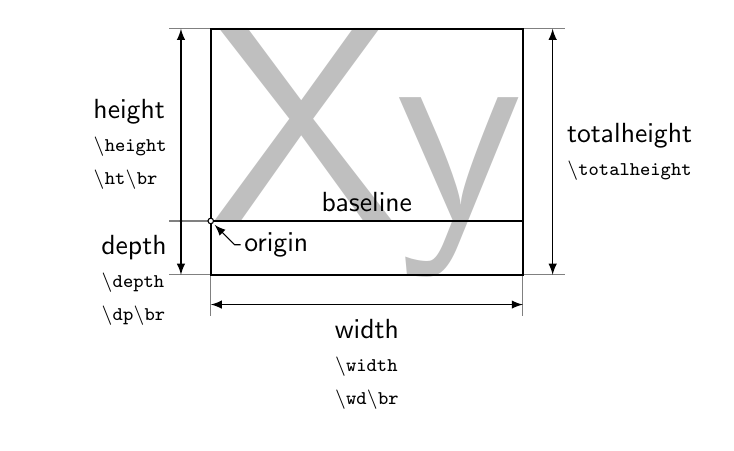
\begin{tikzpicture}[font=\sffamily,>=latex]
   \newcommand\Cs[1]{\texttt{\scriptsize\textbackslash #1}}
   \sbox\mybox{\pgfinterruptpicture\sffamily\color{black!25}\scalebox{10}{Xy}\endpgfinterruptpicture}
   \def\HEIGHT{\ht\mybox}
   \def\WIDTH{\wd\mybox}
   \def\DEPTH{\dp\mybox}
   \draw [gray,thin]
        (0,0)            -- +(-3.5ex,0)
        (0,\HEIGHT)      -- +(-3.5ex,0)
        (0,-\DEPTH)      -- +(-3.5ex,0)
        (\WIDTH,\HEIGHT) -- +(3.5ex,0)
        (\WIDTH,-\DEPTH) -- +(3.5ex,0)
        (0,-\DEPTH)      -- +(0,-3.5ex)
        (\WIDTH,-\DEPTH) -- +(0,-3.5ex)
   ;
   \node [inner sep=0pt,anchor=base west] {\usebox\mybox};
   \draw (0,0) -- (\WIDTH,0) node [above,midway] {baseline};
   \draw [thick] (0,-\DEPTH) rectangle (\WIDTH,\HEIGHT);
   \path [fill=white,draw=black] (0,0) circle (1pt);
   \draw [<-,shorten <=2pt] (0,0) -- (2ex,-2ex) -- +(.5ex,0) node [right=-0.5ex] {origin};
   \tikzset{inner sep=5pt}
   \draw [->] (-2.5ex,0) -- +(0,-\DEPTH)  node [pos=1.1,left,align=left]
        {depth\\\Cs{depth}\\\Cs{dp}\Cs{br}};
   \draw [->] (-2.5ex,0) -- +(0, \HEIGHT) node [pos=.4,left,align=left]
        {height\\\Cs{height}\\\Cs{ht}\Cs{br}};
   \draw [<->] (\WIDTH,-\DEPTH) ++(2.5ex,0) -- +(0,\DEPTH+\HEIGHT) node [midway,right,align=left]
        {totalheight\\\Cs{totalheight}};
   \draw [<->] (0,-\DEPTH) ++(0,-2.5ex) -- +(\WIDTH,0) node [midway,below,align=left]
        {width\\\Cs{width}\\\Cs{wd}\Cs{br}};
   \fill (-2.5ex,0) circle (.5pt);
   \path let
        \p1 = (current bounding box.south west),
        \p2 = (current bounding box.north east),
        \p3 = (0,-\DEPTH),
        \p4 = (\WIDTH,\HEIGHT)
   in
        (\x3-\x2+\x4,\y3) rectangle (\x4+\x3-\x1,\y4);
\end{tikzpicture}
}
%   \caption{Box dimensions. Shown are also the \LaTeX\ macros and the \TeX\ primitives. Here \cs{br} stands for a box register.
%       Note that the depth is a positive values on its own downwards pointed axes.
%   }\label{fig:boxdim}
% \end{figure}
%
% \begin{figure}[!bt]
%   \centering
%   {\catcode`\%=14\relax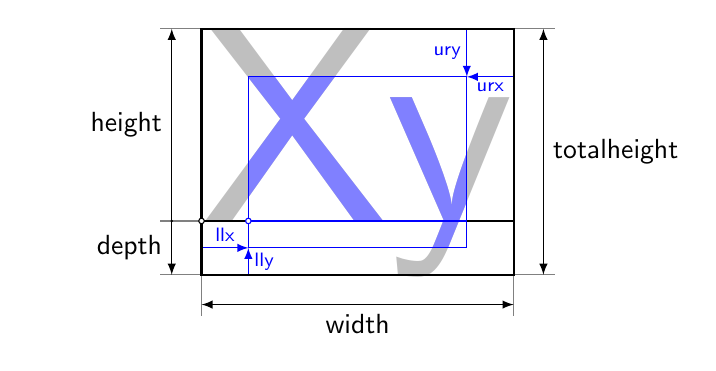
\begin{tikzpicture}[font=\sffamily,>=latex]
   \def\text{\scalebox{10}{Xy}}
   \sbox\mybox{\pgfinterruptpicture\sffamily\color{black!25}\scalebox{10}{Xy}\endpgfinterruptpicture}
   \def\HEIGHT{\ht\mybox}
   \def\WIDTH{\wd\mybox}
   \def\DEPTH{\dp\mybox}
   \def\LLX{.15\WIDTH}
   \def\LLY{.5\DEPTH}
   \def\URX{.15\WIDTH}
   \def\URY{.25\HEIGHT}
   \draw [gray,thin]
        (0,0)       -- +(-3.5ex,0)
        (0,\HEIGHT) -- +(-3.5ex,0)
        (0,-\DEPTH) -- +(-3.5ex,0)
        (\WIDTH,\HEIGHT) -- +(3.5ex,0)
        (\WIDTH,-\DEPTH) -- +(3.5ex,0)
        (0,-\DEPTH)      -- +(0,-3.5ex)
        (\WIDTH,-\DEPTH) -- +(0,-3.5ex)
   ;
   \node [inner sep=0pt,anchor=base west] {\usebox\mybox};
   \draw (0,0) -- (\WIDTH,0);% node [above,midway] {baseline};
   \draw [->] (-2.5ex,0) -- +(0,-\DEPTH)  node [midway,left] {depth};
   \draw [->] (-2.5ex,0) -- +(0, \HEIGHT) node [midway,left] {height};
   \draw [<->] (\WIDTH,-\DEPTH) ++(2.5ex,0) -- +(0,\DEPTH+\HEIGHT) node [midway,right] {totalheight};
   \draw [<->] (0,-\DEPTH) ++(0,-2.5ex) -- +(\WIDTH,0) node [midway,below] {width};
   \fill (-2.5ex,0) circle (.5pt);
   \begin{scope}[blue,every node/.append style={inner sep=2pt}]
    \begin{scope}
        \clip ([shift={(\LLX,\LLY)}]0,-\DEPTH) rectangle ([shift={(-\URX,-\URY)}]\WIDTH,\HEIGHT);
        \node [inner sep=0pt,anchor=base west,color=blue!50!white] {\text};
    \end{scope}
    \draw ([shift={(\LLX,\LLY)}]0,-\DEPTH) rectangle ([shift={(-\URX,-\URY)}]\WIDTH,\HEIGHT);
    \draw [->] (\LLX,-\DEPTH)   -- ++(0,\LLY) node [right,midway] {\scriptsize lly};
    \draw [->] (0,-\DEPTH+\LLY) -- ++(\LLX,0) node [above,midway] {\scriptsize llx};
    \draw (\LLX,0) -- ([shift={(-\URX,0)}]\WIDTH,0);
    \draw [->]
        ([shift={(-\URX,0)}]\WIDTH,\HEIGHT) --
        ([shift={(-\URX,-\URY)}]\WIDTH,\HEIGHT)
        node [left,midway] {\scriptsize ury}
    ;
    \draw [->]
        ([shift={(0,-\URY)}]\WIDTH,\HEIGHT) --
        ([shift={(-\URX,-\URY)}]\WIDTH,\HEIGHT)
        node [below,midway] {\scriptsize urx}
    ;
    \path [fill=white,draw] (\LLX,0) circle (1pt);
   \end{scope}
   \draw [thick] (0,-\DEPTH) rectangle (\WIDTH,\HEIGHT);
   \path [fill=white,draw=black] (0,0) circle (1pt);
   \path let
        \p1 = (current bounding box.south west),
        \p2 = (current bounding box.north east),
        \p3 = (0,-\DEPTH),
        \p4 = (\WIDTH,\HEIGHT)
   in
        (\x3-\x2+\x4,\y3) rectangle (\x4+\x3-\x1,\y4);
\end{tikzpicture}
}
%   \caption{Trimming. The four values are removed from each side.}\label{fig:trim}
% \end{figure}
%
% \begin{figure}
%   \centering
%   {\catcode`\%=14\relax
\def\text{\sffamily\scalebox{10}{Xy}}
\sbox\mybox{\sffamily\color{black!25}\scalebox{10}{Xy}}
\def\HEIGHT{\ht\mybox}
\def\WIDTH{\wd\mybox}
\def\DEPTH{\dp\mybox}
\def\LLX{.15\WIDTH}
\def\LLY{\DEPTH+.15\HEIGHT}
\def\URX{.15\WIDTH}
\def\URY{.25\HEIGHT}
\begin{tikzpicture}[font=\sffamily,>=latex]
   \draw [gray,thin]
        (0,0)       -- +(-3.5ex,0)
        (0,\HEIGHT) -- +(-3.5ex,0)
        (0,-\DEPTH) -- +(-3.5ex,0)
        (\WIDTH,\HEIGHT) -- +(3.5ex,0)
        (\WIDTH,-\DEPTH) -- +(3.5ex,0)
        (0,-\DEPTH)      -- +(0,-3.5ex)
        (\WIDTH,-\DEPTH) -- +(0,-3.5ex)
   ;
   \node [inner sep=0pt,anchor=base west] {\usebox\mybox};
   \draw (0,0) -- (\WIDTH,0);% node [above,midway] {baseline};
   \draw [->] (-2.5ex,0) -- +(0,-\DEPTH)  node [midway,left] {depth};
   \draw [->] (-2.5ex,0) -- +(0, \HEIGHT) node [midway,left] {height};
   \draw [<->] (\WIDTH,-\DEPTH) ++(2.5ex,0) -- +(0,\DEPTH+\HEIGHT) node [midway,right] {totalheight};
   \draw [<->] (0,-\DEPTH) ++(0,-2.5ex) -- +(\WIDTH,0) node [midway,below] {width};
   \fill (-2.5ex,0) circle (.5pt);
   \begin{scope}[blue] %,every node/.append style={inner sep=2pt}]
    \begin{scope}
        \clip ([shift={(\LLX,\LLY)}]0,-\DEPTH) rectangle ([shift={(-\URX,-\URY)}]\WIDTH,\HEIGHT);
        \node [inner sep=0pt,anchor=base west,color=blue!50!white] {\text};
    \end{scope}
    \draw ([shift={(\LLX,\LLY)}]0,-\DEPTH) rectangle ([shift={(-\URX,-\URY)}]\WIDTH,\HEIGHT);
    \draw [->] (\LLX,-\DEPTH)   -- ++(0,\LLY) node [right,midway] {\scriptsize lly};
    \draw [->] (0,-\DEPTH+\LLY) -- ++(\LLX,0) node [above,midway] {\scriptsize llx};
    \draw (\LLX,-\DEPTH+\LLY) -- ([shift={(-\URX,0)}]\WIDTH,-\DEPTH+\LLY);
    \draw [->] (\LLX+.2\WIDTH,-\DEPTH+\LLY) -- (\LLX+.2\WIDTH,0) node [right,midway] {\scriptsize moves down};
    \path [fill=white,draw] (\LLX,-\DEPTH+\LLY) circle (1pt);
    \draw [->]
        ([shift={(-\URX,0)}]\WIDTH,\HEIGHT) --
        ([shift={(-\URX,-\URY)}]\WIDTH,\HEIGHT)
        node [left,midway] {\scriptsize ury}
    ;
    \draw [->]
        ([shift={(0,-\URY)}]\WIDTH,\HEIGHT) --
        ([shift={(-\URX,-\URY)}]\WIDTH,\HEIGHT)
        node [below,midway] {\scriptsize urx}
    ;
   \end{scope}
   \draw [thick] (0,-\DEPTH) rectangle (\WIDTH,\HEIGHT);
   \path [fill=white,draw=black] (0,0) circle (1pt);
   \path let
        \p1 = (current bounding box.south west),
        \p2 = (current bounding box.north east),
        \p3 = (0,-\DEPTH),
        \p4 = (\WIDTH,\HEIGHT)
   in
        (\x3-\x2+\x4,\y3) rectangle (\x4+\x3-\x1,\y4);
\end{tikzpicture}
}
%   \caption{Trimming with \texttt{lly}$>$depth. In this case the resulting box moves up to the original baseline.}\label{fig:trim2}
% \end{figure}
%
% \begin{figure}
%   \centering
%   {\catcode`\%=14\relax
\def\text{\sffamily\scalebox{10}{Xy}}
\sbox\mybox{\sffamily\color{black!25}\scalebox{10}{Xy}}
\def\HEIGHT{\ht\mybox}
\def\WIDTH{\wd\mybox}
\def\DEPTH{\dp\mybox}
\def\LLX{.15\WIDTH}
\def\LLY{.4\DEPTH}
\def\URX{.15\WIDTH}
\def\URY{(\HEIGHT+.25\DEPTH)}
\begin{tikzpicture}[font=\sffamily,>=latex]
   \draw [gray,thin]
        (0,0)       -- +(-3.5ex,0)
        (0,\HEIGHT) -- +(-3.5ex,0)
        (0,-\DEPTH) -- +(-3.5ex,0)
        (\WIDTH,\HEIGHT) -- +(3.5ex,0)
        (\WIDTH,-\DEPTH) -- +(3.5ex,0)
        (0,-\DEPTH)      -- +(0,-3.5ex)
        (\WIDTH,-\DEPTH) -- +(0,-3.5ex)
   ;
   \node [inner sep=0pt,anchor=base west] {\usebox\mybox};
   \draw (0,0) -- (\WIDTH,0);% node [above,midway] {baseline};
   \draw [->] (-2.5ex,0) -- +(0,-\DEPTH)  node [midway,left] {depth};
   \draw [->] (-2.5ex,0) -- +(0, \HEIGHT) node [midway,left] {height};
   \draw [<->] (\WIDTH,-\DEPTH) ++(2.5ex,0) -- +(0,\DEPTH+\HEIGHT) node [midway,right] {totalheight};
   \draw [<->] (0,-\DEPTH) ++(0,-2.5ex) -- +(\WIDTH,0) node [midway,below] {width};
   \fill (-2.5ex,0) circle (.5pt);
   \begin{scope}[blue] %,every node/.append style={inner sep=2pt}]
    \begin{scope}
        \clip ([shift={(\LLX,\LLY)}]0,-\DEPTH) rectangle ([shift={(-\URX,-\URY)}]\WIDTH,\HEIGHT);
        \node [inner sep=0pt,anchor=base west,color=blue!50!white] {\text};
    \end{scope}
    \draw ([shift={(\LLX,\LLY)}]0,-\DEPTH) rectangle ([shift={(-\URX,-\URY)}]\WIDTH,\HEIGHT);
    \draw [->] (\LLX,-\DEPTH)   -- ++(0,\LLY) node [right,midway] {\scriptsize lly};
    \draw [->] (0,-\DEPTH+\LLY) -- ++(\LLX,0) node [above,midway] {\scriptsize llx};
    \draw (\LLX,-\DEPTH+\LLY) -- ([shift={(-\URX,0)}]\WIDTH,-\DEPTH+\LLY);
    \draw [->] (\LLX+.2\WIDTH,{\HEIGHT-\URY}) -- (\LLX+.2\WIDTH,0) node [pos=0.4,below right] {\scriptsize moves up};
    \path [fill=white,draw] (\LLX,{\HEIGHT-\URY}) circle (1pt);
    \draw [->]
        ([shift={(-\URX,0)}]\WIDTH,\HEIGHT) --
        ([shift={(-\URX,-\URY)}]\WIDTH,\HEIGHT)
        node [left,midway] {\scriptsize ury}
    ;
    \draw [->]
        ([shift={(0,-\URY)}]\WIDTH,\HEIGHT) --
        ([shift={(-\URX,-\URY)}]\WIDTH,\HEIGHT)
        node [below,midway] {\scriptsize urx}
    ;
   \end{scope}
   \draw [thick] (0,-\DEPTH) rectangle (\WIDTH,\HEIGHT);
   \path [fill=white,draw=black] (0,0) circle (1pt);
   \path let
        \p1 = (current bounding box.south west),
        \p2 = (current bounding box.north east),
        \p3 = (0,-\DEPTH),
        \p4 = (\WIDTH,\HEIGHT)
   in
        (\x3-\x2+\x4,\y3) rectangle (\x4+\x3-\x1,\y4);
\end{tikzpicture}
}
%   \caption{Trimming with \texttt{ury}$>$height. In this case the resulting box falls down to the original baseline}\label{fig:trim2}
% \end{figure}
%
% \begin{figure}
%   \centering
%   {\catcode`\%=14\relax
\def\text{\sffamily\scalebox{10}{Xy}}
\sbox\mybox{\sffamily\color{black!25}\scalebox{10}{Xy}}
\def\HEIGHT{\ht\mybox}
\def\WIDTH{\wd\mybox}
\def\DEPTH{\dp\mybox}
\def\LLX{.15\WIDTH}
\def\LLY{\DEPTH+.15\HEIGHT}
\def\URX{.15\WIDTH}
\def\URY{.25\HEIGHT}
\begin{tikzpicture}[font=\sffamily,>=latex]
   \draw [gray,thin]
        (0,0)       -- +(-3.5ex,0)
        (0,\HEIGHT) -- +(-3.5ex,0)
        (0,-\DEPTH) -- +(-3.5ex,0)
        (\WIDTH,\HEIGHT) -- +(3.5ex,0)
        (\WIDTH,-\DEPTH) -- +(3.5ex,0)
        (0,-\DEPTH)      -- +(0,-3.5ex)
        (\WIDTH,-\DEPTH) -- +(0,-3.5ex)
   ;
   \node [inner sep=0pt,anchor=base west] {\usebox\mybox};
   \draw (0,0) -- (\WIDTH,0);% node [above,midway] {baseline};
   \draw [->] (-2.5ex,0) -- +(0,-\DEPTH)  node [midway,left] {depth};
   \draw [->] (-2.5ex,0) -- +(0, \HEIGHT) node [midway,left] {height};
   \draw [<->] (\WIDTH,-\DEPTH) ++(2.5ex,0) -- +(0,\DEPTH+\HEIGHT) node [midway,right] {totalheight};
   \draw [<->] (0,-\DEPTH) ++(0,-2.5ex) -- +(\WIDTH,0) node [midway,below] {width};
   \fill (-2.5ex,0) circle (.5pt);
   \begin{scope}[blue]
        \clip ([shift={(\LLX,\LLY)}]0,-\DEPTH) rectangle ([shift={(-\URX,-\URY)}]\WIDTH,\HEIGHT);
        \node [inner sep=0pt,anchor=base west,color=blue!50!white] {\text};
   \end{scope}
   \begin{scope}[blue]
        \draw ([shift={(\LLX,\LLY)}]0,-\DEPTH) rectangle ([shift={(-\URX,-\URY)}]\WIDTH,\HEIGHT);
        \draw (\LLX,-\DEPTH+\LLY) -- ([shift={(-\URX,0)}]\WIDTH,-\DEPTH+\LLY);
        \draw [->] (\LLX+.2\WIDTH,-\DEPTH+\LLY) -- (\LLX+.2\WIDTH,0) node [right,midway] {\scriptsize moves down};
        \path [fill=white,draw] (\LLX,-\DEPTH+\LLY) circle (1pt);
   \end{scope}
   \begin{scope}[blue!50!black] %,every node/.append style={inner sep=2pt}]
    \draw [->] (\LLX,0) -- (\LLX,\LLY-\DEPTH) node [right,midway] {\scriptsize lly};
    \draw [->] (0,-\DEPTH+\LLY) -- ++(\LLX,0) node [above,midway] {\scriptsize llx};
    \draw [->]
        ([shift={(-\URX,0)}]\WIDTH,0) --
        ([shift={(-\URX,-\URY)}]\WIDTH,\HEIGHT)
        node [right,midway] {\scriptsize ury}
    ;
    \draw [->]
        ([shift={(0,-\URY)}]0,\HEIGHT) --
        ([shift={(-\URX,-\URY)}]\WIDTH,\HEIGHT)
        node [above,midway] {\scriptsize urx}
    ;
   \end{scope}
   \draw [thick] (0,-\DEPTH) rectangle (\WIDTH,\HEIGHT);
   \path [fill=white,draw=black] (0,0) circle (1pt);
   \path let
        \p1 = (current bounding box.south west),
        \p2 = (current bounding box.north east),
        \p3 = (0,-\DEPTH),
        \p4 = (\WIDTH,\HEIGHT)
   in
        (\x3-\x2+\x4,\y3) rectangle (\x4+\x3-\x1,\y4);
\end{tikzpicture}
}
%   \caption{Viewport with \texttt{lly}$>$0pt. The \texttt{ll} and \texttt{ur} values are taken from the origin. The baseline is the vertical zero reference.}\label{fig:viewport}
% \end{figure}
%
% \begin{figure}
%   \centering
%   {\catcode`\%=14\relax
\def\text{\sffamily\scalebox{10}{Xy}}
\sbox\mybox{\sffamily\color{black!25}\scalebox{10}{Xy}}
\def\HEIGHT{\ht\mybox}
\def\WIDTH{\wd\mybox}
\def\DEPTH{\dp\mybox}
\def\LLX{.15\WIDTH}
\def\LLY{\DEPTH-.15\HEIGHT}
\def\URX{.15\WIDTH}
\def\URY{.25\HEIGHT}
\begin{tikzpicture}[font=\sffamily,>=latex]
   \draw [gray,thin]
        (0,0)       -- +(-3.5ex,0)
        (0,\HEIGHT) -- +(-3.5ex,0)
        (0,-\DEPTH) -- +(-3.5ex,0)
        (\WIDTH,\HEIGHT) -- +(3.5ex,0)
        (\WIDTH,-\DEPTH) -- +(3.5ex,0)
        (0,-\DEPTH)      -- +(0,-3.5ex)
        (\WIDTH,-\DEPTH) -- +(0,-3.5ex)
   ;
   \node [inner sep=0pt,anchor=base west] {\usebox\mybox};
   \draw (0,0) -- (\WIDTH,0);% node [above,midway] {baseline};
   \draw [->] (-2.5ex,0) -- +(0,-\DEPTH)  node [midway,left] {depth};
   \draw [->] (-2.5ex,0) -- +(0, \HEIGHT) node [midway,left] {height};
   \draw [<->] (\WIDTH,-\DEPTH) ++(2.5ex,0) -- +(0,\DEPTH+\HEIGHT) node [midway,right] {totalheight};
   \draw [<->] (0,-\DEPTH) ++(0,-2.5ex) -- +(\WIDTH,0) node [midway,below] {width};
   \fill (-2.5ex,0) circle (.5pt);
   \begin{scope}[blue]
        \clip ([shift={(\LLX,\LLY)}]0,-\DEPTH) rectangle ([shift={(-\URX,-\URY)}]\WIDTH,\HEIGHT);
        \node [inner sep=0pt,anchor=base west,color=blue!50!white] {\text};
   \end{scope}
   \begin{scope}[blue]
        \draw ([shift={(\LLX,\LLY)}]0,-\DEPTH) rectangle ([shift={(-\URX,-\URY)}]\WIDTH,\HEIGHT);
        \draw (\LLX,0) -- ([shift={(-\URX,0)}]\WIDTH,0);
        \path [fill=white,draw] (\LLX,0) circle (1pt);
   \end{scope}
   \begin{scope}[blue!50!black] %,every node/.append style={inner sep=2pt}]
    \draw [->] (\LLX,0) -- (\LLX,\LLY-\DEPTH) node [right,midway] {\scriptsize lly};
    \draw [->] (0,-\DEPTH+\LLY) -- ++(\LLX,0) node [above,midway] {\scriptsize llx};
    \draw [->]
        ([shift={(-\URX,0)}]\WIDTH,0) --
        ([shift={(-\URX,-\URY)}]\WIDTH,\HEIGHT)
        node [right,midway] {\scriptsize ury}
    ;
    \draw [->]
        ([shift={(0,-\URY)}]0,\HEIGHT) --
        ([shift={(-\URX,-\URY)}]\WIDTH,\HEIGHT)
        node [above,midway] {\scriptsize urx}
    ;
   \end{scope}
   \draw [thick] (0,-\DEPTH) rectangle (\WIDTH,\HEIGHT);
   \path [fill=white,draw=black] (0,0) circle (1pt);
   \path let
        \p1 = (current bounding box.south west),
        \p2 = (current bounding box.north east),
        \p3 = (0,-\DEPTH),
        \p4 = (\WIDTH,\HEIGHT)
   in
        (\x3-\x2+\x4,\y3) rectangle (\x4+\x3-\x1,\y4);
\end{tikzpicture}
}
%   \caption{Viewport with \texttt{lly}$<$0pt. In this case the viewport ranges into the depth of the original box.}
% \end{figure}
%
% \begin{figure}
%   \centering
%   {\catcode`\%=14\relax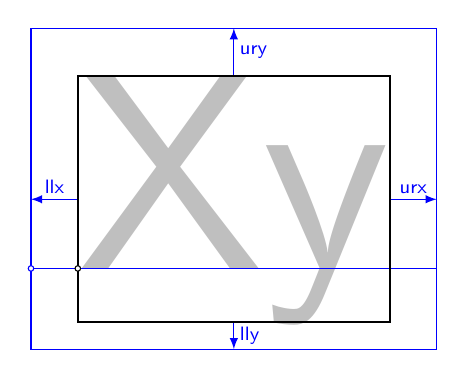
\begin{tikzpicture}[font=\sffamily,>=latex]
   \def\text{\scalebox{10}{Xy}}
   \sbox\mybox{\pgfinterruptpicture\sffamily\color{black!25}\scalebox{10}{Xy}\endpgfinterruptpicture}
   \def\HEIGHT{\ht\mybox}
   \def\WIDTH{\wd\mybox}
   \def\DEPTH{\dp\mybox}
   \def\LLX{.15\WIDTH}
   \def\LLY{.5\DEPTH}
   \def\URX{.15\WIDTH}
   \def\URY{.25\HEIGHT}
   \node [inner sep=0pt,anchor=base west] {\usebox\mybox};
   \draw (0,0) -- (\WIDTH,0);% node [above,midway] {baseline};
   \begin{scope}[blue,every node/.append style={inner sep=2pt}]
    \begin{scope}
        \draw ([shift={(-\LLX,-\LLY)}]0,-\DEPTH) rectangle ([shift={(\URX,\URY)}]\WIDTH,\HEIGHT);
    \end{scope}
    \draw [->] (.5\WIDTH,-\DEPTH) -- ++(0,-\LLY) node [right,midway] {\scriptsize lly};
    \draw [->] (0,.5*\HEIGHT-.5*\DEPTH) -- ++(-\LLX,0) node [above,midway] {\scriptsize llx};
    \draw (-\LLX,0) -- ([shift={(+\URX,0)}]\WIDTH,0);
    \draw [->] (.5\WIDTH,\HEIGHT) -- ++(0,\URY) node [right,midway] {\scriptsize ury};
    \draw [->] (\WIDTH,.5*\HEIGHT-.5*\DEPTH) -- ++(\URX,0) node [above,midway] {\scriptsize urx};
    \path [fill=white,draw] (-\LLX,0) circle (1pt);
   \end{scope}
   \draw [thick] (0,-\DEPTH) rectangle (\WIDTH,\HEIGHT);
   \path [fill=white,draw=black] (0,0) circle (1pt);
   \path let
        \p1 = (current bounding box.south west),
        \p2 = (current bounding box.north east),
        \p3 = (0,-\DEPTH),
        \p4 = (\WIDTH,\HEIGHT)
   in
        (\x3-\x2+\x4,\y3) rectangle (\x4+\x3-\x1,\y4);
\end{tikzpicture}
}
%   \caption{Marginbox. The \texttt{llx} and \texttt{urx} are added to the left and right and increase the width. The \texttt{ury} is added to the height
%   and \texttt{lly} to the depth of the box. This keeps the baseline at the original position.}
%   \label{fig:margin}
% \end{figure}
%
% \begin{figure}
%   \centering
%   {\catcode`\%=14\relax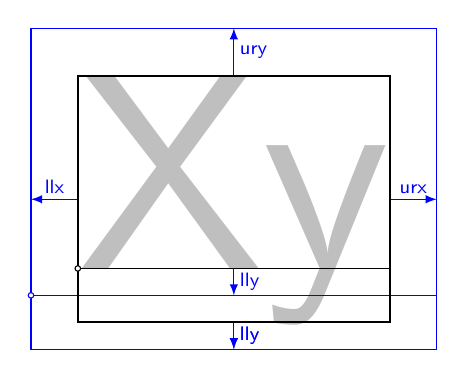
\begin{tikzpicture}[font=\sffamily,>=latex]
   \def\text{\scalebox{10}{Xy}}
   \sbox\mybox{\pgfinterruptpicture\sffamily\color{black!25}\scalebox{10}{Xy}\endpgfinterruptpicture}
   \def\HEIGHT{\ht\mybox}
   \def\WIDTH{\wd\mybox}
   \def\DEPTH{\dp\mybox}
   \def\LLX{.15\WIDTH}
   \def\LLY{.5\DEPTH}
   \def\URX{.15\WIDTH}
   \def\URY{.25\HEIGHT}
   \node [inner sep=0pt,anchor=base west] {\usebox\mybox};
   \draw (0,0) -- (\WIDTH,0);% node [above,midway] {baseline};
   \begin{scope}[blue,every node/.append style={inner sep=2pt}]
    \begin{scope}
        \draw ([shift={(-\LLX,-\LLY)}]0,-\DEPTH) rectangle ([shift={(\URX,\URY)}]\WIDTH,\HEIGHT);
    \end{scope}
    \draw [->] (.5\WIDTH,-\DEPTH) -- ++(0,-\LLY) node [right,midway] {\scriptsize lly};
    \draw [->] (0,.5*\HEIGHT-.5*\DEPTH) -- ++(-\LLX,0) node [above,midway] {\scriptsize llx};
    \draw [->] (.5\WIDTH,\HEIGHT) -- ++(0,\URY) node [right,midway] {\scriptsize ury};
    \draw [->] (\WIDTH,.5*\HEIGHT-.5*\DEPTH) -- ++(\URX,0) node [above,midway] {\scriptsize urx};
    \draw [->] (.5\WIDTH,-\DEPTH) -- ++(0,-\LLY) node [right,midway] {\scriptsize lly};
    \draw (-\LLX,-\LLY) -- ([shift={(+\URX,0)}]\WIDTH,-\LLY);
    \path [fill=white,draw] (-\LLX,-\LLY) circle (1pt);
    \draw [->] (.5\WIDTH,0pt) -- ++(0,-\LLY) node [right,midway] {\scriptsize lly};
   \end{scope}
   \draw [thick] (0,-\DEPTH) rectangle (\WIDTH,\HEIGHT);
   \path [fill=white,draw=black] (0,0) circle (1pt);
   \path let
        \p1 = (current bounding box.south west),
        \p2 = (current bounding box.north east),
        \p3 = (0,-\DEPTH),
        \p4 = (\WIDTH,\HEIGHT)
   in
        (\x3-\x2+\x4,\y3) rectangle (\x4+\x3-\x1,\y4);
\end{tikzpicture}
}
%   \caption{Marginbox*. In addition to the normal margin the content
%   is also raised by \texttt{lly}, so that the original depth is preserved.
%   This effectively moves the baseline down.}
%   \label{fig:margin}
% \end{figure}
%
% \StopEventually{}
% \clearpage
% \section{Implementation}
% \setcounter{lstnumber}{1}
%
%
% \iffalse
%<*trimclip.sty>
% \fi
%    \begin{macrocode}
%<!COPYRIGHT>
\ProvidesPackage{trimclip}[%
%<!DATE>
%<!VERSION>
%<*DRIVER>
    2099/01/01 develop
%</DRIVER>
    Trim and clip general TeX material]
%    \end{macrocode}
%
%
% %%%%%%%%%%%%%%%%%%%%%%%%%%%%%%%%%%%%%%%%%%%%%%%%%%%%%%%%%%%%%%%%%%%%%%%%%%%%%%%%%%%%%%%%%%%%%%%%%%%%%%%%%%%%%%%%%%%%%
% \subsection{Options}
% %%%%%%%%%%%%%%%%%%%%%%%%%%%%%%%%%%%%%%%%%%%%%%%%%%%%%%%%%%%%%%%%%%%%%%%%%%%%%%%%%%%%%%%%%%%%%%%%%%%%%%%%%%%%%%%%%%%%%
%    \begin{macrocode}
\def\tc@driver{tc-\Gin@driver}
\DeclareOption{pgf}{\def\tc@driver{tc-pgf.def}\PassOptionsToPackage{pgf}{graphicx}}
\DeclareOption{pdftex}{\def\tc@driver{tc-pdftex.def}\PassOptionsToPackage{pdftex}{graphicx}}
\DeclareOption{xetex}{\def\tc@driver{tc-xetex.def}\PassOptionsToPackage{xetex}{graphicx}}
\DeclareOption{dvips}{\def\tc@driver{tc-dvips.def}\PassOptionsToPackage{dvips}{graphicx}}
\DeclareOption{dvipdfm}{\def\tc@driver{tc-xetex.def}\PassOptionsToPackage{xetex}{graphicx}}
\DeclareOption{dvipdf}{\def\tc@driver{tc-xetex.def}\PassOptionsToPackage{xetex}{graphicx}}
\DeclareOption*{%
    \@ifpackageloaded{graphics}{%
        \edef\tc@driver{tc-\CurrentOption.def}%
        \begingroup
        \edef\@tempa{\CurrentOption.def}%
        \ifx\@tempa\Gin@driver\else
            \let\on@line\@gobble
            \PackageWarning{trimclip}{%
                A different clipping driver was requested than the\MessageBreak
                one used for 'graphics/x'! This is not recommended\MessageBreak
                and can lead to defect output files.%
            }%
        \fi
        \endgroup
    }{%
        \def\tc@driver{tc-\Gin@driver}%
        \PassOptionsToPackage\CurrentOption{graphicx}%
    }%
}
\ProcessOptions*\relax
%    \end{macrocode}
%
%    \begin{macrocode}
\RequirePackage{graphicx}[1999/02/16]
\RequirePackage{collectbox}[2011/08/22]
\RequirePackage{adjcalc}
%    \end{macrocode}
%
%
% %%%%%%%%%%%%%%%%%%%%%%%%%%%%%%%%%%%%%%%%%%%%%%%%%%%%%%%%%%%%%%%%%%%%%%%%%%%%%%%%%%%%%%%%%%%%%%%%%%%%%%%%%%%%%%%%%%%%%
% \subsection{User level and auxiliary macros}
% %%%%%%%%%%%%%%%%%%%%%%%%%%%%%%%%%%%%%%%%%%%%%%%%%%%%%%%%%%%%%%%%%%%%%%%%%%%%%%%%%%%%%%%%%%%%%%%%%%%%%%%%%%%%%%%%%%%%%
%
% \begin{macro}{\tc@readvalues}
% Reads the four values for trim, viewport and clip.
% Valid inputs are:
%  4 values directly,
%  1 value which is taken four times,
%  2 values which is taken for left/right and top/bottom.
%    \begin{macrocode}
\def\tc@readvalues#1{%
    \tc@@readvalues#1 {} {} {} \\%
}
%    \end{macrocode}
% \end{macro}
%
%
% \begin{macro}{\tc@@readvalues}
%    \begin{macrocode}
\def\tc@@readvalues#1 #2 #3 #4 #5\\{%
  \adjsetlengthdefault\tc@llx{#1}%
  \ifx\@nnil#2\@nnil
    \tc@lly\tc@llx
    \tc@urx\tc@llx
    \tc@ury\tc@llx
  \else
    \adjsetlengthdefault\tc@lly{#2}%
    \ifx\@nnil#3\@nnil
      \tc@urx\tc@llx
      \tc@ury\tc@lly
    \else
      \adjsetlengthdefault\tc@urx{#3}%
      \adjsetlengthdefault\tc@ury{#4}%
    \fi
  \fi
}%
%    \end{macrocode}
% \end{macro}
%
%
% \begin{macro}{\tc@llx}
% \begin{macro}{\tc@lly}
% \begin{macro}{\tc@urx}
% \begin{macro}{\tc@ury}
% Dimension registers for the four trim/viewport values.
% Legend: ll = lower left, ur = upper right.
%    \begin{macrocode}
\newdimen\tc@llx
\newdimen\tc@lly
\newdimen\tc@urx
\newdimen\tc@ury
%    \end{macrocode}
% \end{macro}
% \end{macro}
% \end{macro}
% \end{macro}
%
%
% \begin{macro}{\trimbox}
%    \begin{macrocode}
\newcommand\trimbox{%
    \collectboxcheckenv{trimbox}%
    \@ifstar
        \trimbox@s
        \trimbox@
}
\def\trimbox@#1{%
    \collectbox{\@trimclip\@trimbox{#1}}%
}
\def\trimbox@s#1{%
    \collectbox{\@trimclip\@viewportbox{#1}}%
}
%    \end{macrocode}
% \end{macro}
%
%
% \begin{environment}{trimbox*}
%    \begin{macrocode}
\expandafter\newcommand\expandafter*\csname trimbox*\endcsname{%
    \@collectboxisenv{trimbox*}%
    \trimbox@s
}
%    \end{macrocode}
% \end{environment}
%
%
% \begin{macro}{\clipbox}
%    \begin{macrocode}
\newcommand\clipbox{%
    \collectboxcheckenv{clipbox}%
    \@ifstar
        \clipbox@s
        \clipbox@
}
\def\clipbox@#1{%
    \collectbox{\@trimclip\@clipbox{#1}}%
}
\def\clipbox@s#1{%
    \collectbox{\@trimclip\@clipvpbox{#1}}%
}
%    \end{macrocode}
% \end{macro}
%
%
% \begin{environment}{clipbox*}
%    \begin{macrocode}
\expandafter\newcommand\expandafter*\csname clipbox*\endcsname{%
    \@collectboxisenv{clipbox*}%
    \clipbox@s
}
%    \end{macrocode}
% \end{environment}
%
%
% \begin{macro}{\marginbox}[1]{Margins as space separated values (like for 'trim')}
% Collect box first.
%    \begin{macrocode}
\newcommand\marginbox{%
    \collectboxcheckenv{marginbox}%
    \@ifstar
        \marginbox@s
        \marginbox@
}
\def\marginbox@#1{%
    \@collectbox{\@trimclip\@marginbox{#1}}%
}
\def\marginbox@s#1{%
    \@collectbox{\@trimclip\@marginraisebox{#1}}%
}
%    \end{macrocode}
% \end{macro}
%
%
% \begin{environment}{marginbox*}[1]{Margins as space separated values (like for 'trim')}
%    \begin{macrocode}
\expandafter\newcommand\expandafter*\csname marginbox*\endcsname{%
    \@collectboxisenv{marginbox*}%
    \marginbox@s
}
%    \end{macrocode}
% \end{environment}
%
%
% \begin{macro}{\@trimclip}[2]{<trim/viewport/clip macro>}{<values>}
% General macro which parses the values and feeds it to the given lower-level macro.
% Finally the box is typeset. This macro will always be used inside a group
% created by \Macro\@collectbox.
%    \begin{macrocode}
\def\@trimclip#1#2{%
    \tc@readvalues{#2}%
    #1%
        \collectedbox
        \tc@llx
        \tc@lly
        \tc@urx
        \tc@ury
    \usebox\collectedbox
}
%    \end{macrocode}
% \end{macro}
%
%
%
% %%%%%%%%%%%%%%%%%%%%%%%%%%%%%%%%%%%%%%%%%%%%%%%%%%%%%%%%%%%%%%%%%%%%%%%%%%%%%%%%%%%%%%%%%%%%%%%%%%%%%%%%%%%%%%%%%%%%%
% \subsection{Low-level commands}
% %%%%%%%%%%%%%%%%%%%%%%%%%%%%%%%%%%%%%%%%%%%%%%%%%%%%%%%%%%%%%%%%%%%%%%%%%%%%%%%%%%%%%%%%%%%%%%%%%%%%%%%%%%%%%%%%%%%%%
%
%
% \begin{macro}{\tc@correctbaseline}
% Adjust baseline if required by negative depth or height.
%    \begin{macrocode}
\def\tc@correctbaseline#1{%
%    \end{macrocode}
% If depth is negative lower the box to get zero depth
%    \begin{macrocode}
    \ifdim\dp#1<\z@
        \raise\dp#1%
    \else
%    \end{macrocode}
% Else if height is negative lower the box to get zero height
%    \begin{macrocode}
    \ifdim\ht#1<\z@
        \lower\ht#1%
    \fi\fi
    \box#1%
}%
%    \end{macrocode}
% \end{macro}
%
%
% \begin{macro}{\tc@correctdims}
% Ensure that all dimensions are non-negative.
%    \begin{macrocode}
\def\tc@correctdims#1{%
    \ifdim\dp#1<\z@ \dp#1=\z@ \fi
    \ifdim\wd#1<\z@ \wd#1=\z@ \fi
    \ifdim\ht#1<\z@ \ht#1=\z@ \fi
}
%    \end{macrocode}
% \end{macro}
%
%
% \begin{macro}{\@trimbox}[5]{<box register>}{<tllx>}{<tlly>}{<turx>}{<tury>}
% Removes the four length for the left, bottom, right and top from the official size of the box register.
%    \begin{macrocode}
\def\@trimbox#1#2#3#4#5{%
    \setbox#1=\hbox{%
        %
        \tc@llx=#2\relax
        \tc@lly=#3\relax
        \advance\tc@lly-\dp#1%
        \tc@urx=#4\relax
        \advance\tc@urx-\wd#1%
        \tc@ury=#5\relax
        \advance\tc@ury-\ht#1%
        %
        % Set dimensions now.
        % This allows that the arguments can refer
        % to the original dimensions without issues.
        \hskip-\tc@llx
        \dp#1-\tc@lly
        \wd#1-\tc@urx
        \ht#1-\tc@ury
        %
        \tc@correctbaseline{#1}%
    }%
    \tc@correctdims{#1}%
}
%    \end{macrocode}
% \end{macro}
%
%
%
% \begin{macro}{\@marginbox}
% Adds the given margins to the depth, width and height.
% The left margin is created by an horizontal skip.
% This implementation assumes that the margins are positive and no special checks are added.
% While negative margins will trim some margin off, this will not lead to correct results if this amounts
% are larger than the existing dimensions. For this the \Macro\@trimbox macro should be used.
%    \begin{macrocode}
\def\@marginbox#1#2#3#4#5{%
    \setbox#1=\hbox{%
        %
        \tc@llx=#2\relax
        \tc@lly=#3\relax
        \advance\tc@lly\dp#1%
        \tc@urx=#4\relax
        \advance\tc@urx\wd#1%
        \tc@ury=#5\relax
        \advance\tc@ury\ht#1%
        %
        % Set dimensions now.
        % This allows that the arguments can refer
        % to the original dimensions without issues.
        \hskip\tc@llx
        \dp#1\tc@lly
        \wd#1\tc@urx
        \ht#1\tc@ury
        %
        \box#1%
    }%
    \tc@correctdims{#1}%
}
%    \end{macrocode}
% \end{macro}
%
% \begin{macro}{\@marginraisebox}
% Like \Macro\@marginbox but raises the box accordant to the bottom margin,
% so that the original depth is kept.
%    \begin{macrocode}
\def\@marginraisebox#1#2#3#4#5{%
    \setbox#1=\hbox{%
        %
        \tc@llx=#2\relax
        \tc@lly=#3\relax
        \tc@urx=#4\relax
        \advance\tc@urx\wd#1%
        \tc@ury=#5\relax
        \advance\tc@ury\ht#1%
        %
        % Set dimensions now.
        % This allows that the arguments can refer
        % to the original dimensions without issues.
        \hskip\tc@llx
        \wd#1\tc@urx
        \ht#1\tc@ury
        % Copy original tty values (ury is taken as temp dimension)
        \tc@ury=\tc@lly
        \advance\tc@lly\dp#1%
        \dp#1\tc@lly
        % Raise bu original tty value (now in ury)
        \raise\tc@ury\box#1%
    }%
    \tc@correctdims{#1}%
}
%    \end{macrocode}
% \end{macro}
%
% \begin{macro}{\@trimbox}[5]{<box register>}{<tllx>}{<tlly>}{<turx>}{<tury>}
% Removes the four length for the left, bottom, right and top from the official size of the box register.
%    \begin{macrocode}
\def\@viewportbox#1#2#3#4#5{%
    \setbox#1=\hbox{%
        %
        % Assign values
        \tc@llx=#2\relax
        \tc@lly=#3\relax
        \tc@urx=#4\relax
        \tc@ury=#5\relax
        %
        % Set dimensions now.
        % This allows that the arguments can refer
        % to the original dimensions without issues.
        \hskip-\tc@llx
        \dp#1-\tc@lly
        \wd#1\tc@urx
        \ht#1\tc@ury
        %
        \tc@correctbaseline{#1}%
    }%
    \tc@correctdims{#1}%
}
%    \end{macrocode}
% \end{macro}
%
%
% \begin{macro}{\@clipbox}
% Clips the box using the given trim amounts.
% For this the box is first trimmed and then clipped to its official size using a driver dependent macro.
%    \begin{macrocode}
\def\@clipbox#1#2#3#4#5{%
    \@trimbox{#1}{#2}{#3}{#4}{#5}%
    \@cliptoboxdim{#1}%
}
%    \end{macrocode}
% \end{macro}
%
%
% \begin{macro}{\@clipvpbox}
% Clips the box using the given trim amounts.
% For this the box is first trimmed and then clipped to its official size using a driver dependent macro.
%    \begin{macrocode}
\def\@clipvpbox#1#2#3#4#5{%
    \@viewportbox{#1}{#2}{#3}{#4}{#5}%
    \@cliptoboxdim{#1}%
}
%    \end{macrocode}
% \end{macro}
%
%
%
% %%%%%%%%%%%%%%%%%%%%%%%%%%%%%%%%%%%%%%%%%%%%%%%%%%%%%%%%%%%%%%%%%%%%%%%%%%%%%%%%%%%%%%%%%%%%%%%%%%%%%%%%%%%%%%%%%%%%%
% \subsection{Driver loading}
% %%%%%%%%%%%%%%%%%%%%%%%%%%%%%%%%%%%%%%%%%%%%%%%%%%%%%%%%%%%%%%%%%%%%%%%%%%%%%%%%%%%%%%%%%%%%%%%%%%%%%%%%%%%%%%%%%%%%%
% The clipping support is output driver dependent. The driver selected by \pkg{graphics} is used and a definition file
% is used if its exists. Otherwise either the default \texttt{pdftex} implementation or the \pkg{pgf} fall-back driver
% is used.
%    \begin{macrocode}
\InputIfFileExists{\tc@driver}{%
    {\let\on@line\@gobble
    \PackageInfo{trimclip}{Using driver '\tc@driver'.}}%
}{%
    %% Copyright (C) 2011-2012 by Martin Scharrer <martin@scharrer-online.de>
%% ----------------------------------------------------------------------
%% This work may be distributed and/or modified under the
%% conditions of the LaTeX Project Public License, either version 1.3
%% of this license or (at your option) any later version.
%% The latest version of this license is in
%%   http://www.latex-project.org/lppl.txt
%% and version 1.3 or later is part of all distributions of LaTeX
%% version 2005/12/01 or later.
%%
%% This work has the LPPL maintenance status `maintained'.
%%
%% The Current Maintainer of this work is Martin Scharrer.
%%
%% This work consists of the files trimclip.dtx, adjustbox.ins
%% and the derived files trimclip.sty,
%% tc-dvips.def, tc-pdftex.def, tc-pgf.def and tc-xetex.def.
%% Further author information are located in the .def files.
%%
\ProvidesFile{tc-pgf.def}[2012/05/13 v1.0 trimclip fall-back clipping driver using PGF]
\RequirePackage{pgf}
\def\@cliptoboxdim#1{%
    \setbox#1\hbox{\begin{pgfpicture}%
        \pgfpathmoveto{\pgfqpoint\z@{-\dp#1}}%
        \pgfpathlineto{\pgfqpoint\z@{\ht#1}}%
        \pgfpathlineto{\pgfqpoint{\wd#1}{\ht#1}}%
        \pgfpathlineto{\pgfqpoint{\wd#1}{-\dp#1}}%
        \pgfpathclose
        \pgfusepathqclip
        \pgfset{inner sep=\z@,outer sep=\z@,minimum size=\z@}%
        \pgfnode{rectangle}{base west}{\usebox#1}{}{}%
        \pgfsetbaselinepointnow{\pgfpoint\z@\z@}%
    \end{pgfpicture}}%
}
\endinput
%%
%% End of file `tc-pgf.def'.
%
    {\let\on@line\@gobble
    \PackageInfo{trimclip}{No clipping driver '\tc@driver' available.\MessageBreak Using fall-back PGF driver.}}%
}
%    \end{macrocode}
%
%
% \iffalse
%</trimclip.sty>
% \fi
%
% \subsection{Driver files}
%
% \subsubsection{PGF fall-back driver}
% \iffalse
%<*tc-pgf.def>
% \fi
%    \begin{macrocode}
%<!COPYRIGHT>
\ProvidesFile{tc-pgf.def}[2012/05/13 v1.0 trimclip fall-back clipping driver using PGF]
%    \end{macrocode}
%
%    \begin{macrocode}
\RequirePackage{pgf}
%    \end{macrocode}
%
% \begin{macro}{\@cliptoboxdim}
% Clips to official box dimension.
%    \begin{macrocode}
\def\@cliptoboxdim#1{%
    \setbox#1\hbox{\begin{pgfpicture}%
        \pgfpathmoveto{\pgfqpoint\z@{-\dp#1}}%
        \pgfpathlineto{\pgfqpoint\z@{\ht#1}}%
        \pgfpathlineto{\pgfqpoint{\wd#1}{\ht#1}}%
        \pgfpathlineto{\pgfqpoint{\wd#1}{-\dp#1}}%
        \pgfpathclose
        \pgfusepathqclip
        \pgfset{inner sep=\z@,outer sep=\z@,minimum size=\z@}%
        \pgfnode{rectangle}{base west}{\usebox#1}{}{}%
        \pgfsetbaselinepointnow{\pgfpoint\z@\z@}%
    \end{pgfpicture}}%
}
%    \end{macrocode}
% \end{macro}
%
%^^A vim: ft=tex
% \iffalse
%</tc-pgf.def>
% \fi
%
% \subsubsection{pdftex driver}
% \iffalse
%<*tc-pdftex.def>
% \fi
%    \begin{macrocode}
%<!COPYRIGHT>
\ProvidesFile{tc-pdftex.def}[2012/05/13 v1.0 Clipping driver for pdftex]
%    \end{macrocode}
%
% \begin{macro}{\@cliptoboxdim}
% Clips to official box dimension.
%
% Uses now \Macro\pdfliteral because \Macro\pdfxform does not support
% transparencies and patterns with TikZ.
%    \begin{macrocode}
\def\@cliptoboxdim#1{%
    \setbox#1=\hbox{%
        \Gin@defaultbp\WIDTH{\wd#1}%
        \Gin@defaultbp\DEPTH{\dp#1}%
        \@tempdima\ht#1%
        \advance\@tempdima\dp#1%
        \Gin@defaultbp\TOTALHEIGHT{\@tempdima}%
        \pdfsave
            \pdfliteral direct {%
                0 -\DEPTH\space \WIDTH\space \TOTALHEIGHT\space re W n
            }%
            \hbox to 0pt{\copy#1\hss}%
        \pdfrestore
        \hskip \wd#1
    }%
}
%    \end{macrocode}
% \end{macro}
%
%^^A vim: ft=tex
% \iffalse
%</tc-pdftex.def>
% \fi
%
% \subsubsection{dvips driver}
% \iffalse
%<*tc-dvips.def>
% \fi
%    \begin{macrocode}
%<!COPYRIGHT>
\ProvidesFile{tc-dvips.def}[2012/05/13 v1.0 Clipping driver for dvips]
%    \end{macrocode}
%
% \begin{macro}{\@cliptoboxdim}[1]{box register to clip}
% Clips to official box dimension.
%
% The following clipping code was suggested by
% Joseph Wright (LaTeX3 project), but slightly modified
% for this package.
%    \begin{macrocode}
\def\@cliptoboxdim#1{%
    \setbox#1=\hbox{%
        \adjsetlength\@tempdima{\ht#1+\dp#1}%
        \edef\TOTALHEIGHT{-\strip@pt\@tempdima\space}%
        \edef\DEPTH{\strip@pt\dp#1\space}%
        \edef\WIDTH{\strip@pt\wd#1\space}%
        \special{%
            ps:
              /mtrxc matrix currentmatrix def
              currentpoint gsave
              translate
              Resolution 72 div VResolution 72 div
              scale
              newpath
              0 \DEPTH \WIDTH \TOTALHEIGHT rectclip
              newpath
              mtrxc setmatrix
        }%
        \box#1%
        \special{ps: grestore }%
    }%
}
%    \end{macrocode}
% \end{macro}
%
%^^A vim: ft=tex
% \iffalse
%</tc-dvips.def>
% \fi
%
% \subsubsection{xetex driver}
% \iffalse
%<*tc-xetex.def>
% \fi
%    \begin{macrocode}
%<!COPYRIGHT>
\ProvidesFile{tc-xetex.def}[2012/05/13 v1.0 Clipping driver for xetex]
%    \end{macrocode}
%
% \begin{macro}{\@cliptoboxdim}
% Clips to official box dimension.
%
% The following clipping code was suggested by
% Joseph Wright (LaTeX3 project), but slightly modified
% for this package.
%    \begin{macrocode}
\def\@cliptoboxdim#1{%
    \setbox#1=\hbox{%
        \Gin@defaultbp\WIDTH{\wd#1}%
        \Gin@defaultbp\DEPTH{\dp#1}%
        \@tempdima\ht#1%
        \advance\@tempdima\dp#1%
        \Gin@defaultbp\TOTALHEIGHT{\@tempdima}%
        \special{pdf:bcontent }%
        \special{%
            pdf:literal direct
                0 -\DEPTH\space \WIDTH\space \TOTALHEIGHT\space re
        }%
        \special{pdf:literal direct W }%
        \special{pdf:literal direct n }%
            \box#1%
        \special{pdf:econtent }%
    }%
}
%    \end{macrocode}
% \end{macro}
%
%^^A vim: ft=tex
% \iffalse
%</tc-xetex.def>
% \fi
%
% \Finale
% \endinput
%
% ^^A Standalone figures:
%
% \iffalse
%<*box.tex>
% \fi
%<*standalone>
\documentclass{standalone}

\usepackage{tikz}
\usetikzlibrary{calc}
\newsavebox\mybox

\begin{document}
%</standalone>
% Diagram of the TeX box model and its dimensions
% Copyright (C) 2001 by Martin Scharrer <martin@scharrer.me>, Nov 12th 2011
% This is free code under the LPPL v1.3 or later version OR the CC BY-SA 3.0
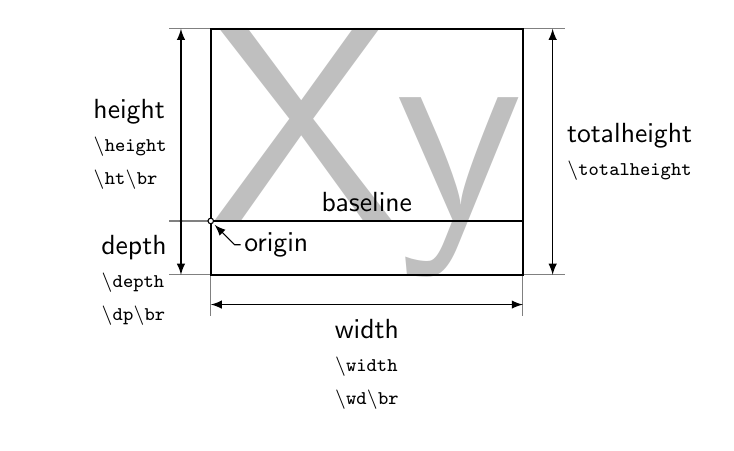
\begin{tikzpicture}[font=\sffamily,>=latex]
   \newcommand\Cs[1]{\texttt{\scriptsize\textbackslash #1}}
% Save example text in box
   \sbox\mybox{\pgfinterruptpicture\sffamily\color{black!25}\scalebox{10}{Xy}\endpgfinterruptpicture}
   \def\HEIGHT{\ht\mybox}
   \def\WIDTH{\wd\mybox}
   \def\DEPTH{\dp\mybox}
% Extensions lines for dimensions (drawn here to be below other material)
   \draw [gray,thin]
        (0,0)            -- +(-3.5ex,0)
        (0,\HEIGHT)      -- +(-3.5ex,0)
        (0,-\DEPTH)      -- +(-3.5ex,0)
        (\WIDTH,\HEIGHT) -- +(3.5ex,0)
        (\WIDTH,-\DEPTH) -- +(3.5ex,0)
        (0,-\DEPTH)      -- +(0,-3.5ex)
        (\WIDTH,-\DEPTH) -- +(0,-3.5ex)
   ;
% Text node:
   \node [inner sep=0pt,anchor=base west] {\usebox\mybox};
% Baseline
   \draw (0,0) -- (\WIDTH,0) node [above,midway] {baseline};
% Box
   \draw [thick] (0,-\DEPTH) rectangle (\WIDTH,\HEIGHT);
% Origin
   \path [fill=white,draw=black] (0,0) circle (1pt);
   \draw [<-,shorten <=2pt] (0,0) -- (2ex,-2ex) -- +(.5ex,0) node [right=-0.5ex] {origin};
% Dimensions
   \tikzset{inner sep=5pt}
   \draw [->] (-2.5ex,0) -- +(0,-\DEPTH)  node [pos=1.1,left,align=left]
        {depth\\\Cs{depth}\\\Cs{dp}\Cs{br}};
   \draw [->] (-2.5ex,0) -- +(0, \HEIGHT) node [pos=.4,left,align=left]
        {height\\\Cs{height}\\\Cs{ht}\Cs{br}};
   \draw [<->] (\WIDTH,-\DEPTH) ++(2.5ex,0) -- +(0,\DEPTH+\HEIGHT) node [midway,right,align=left]
        {totalheight\\\Cs{totalheight}};
   \draw [<->] (0,-\DEPTH) ++(0,-2.5ex) -- +(\WIDTH,0) node [midway,below,align=left]
        {width\\\Cs{width}\\\Cs{wd}\Cs{br}};
   \fill (-2.5ex,0) circle (.5pt);
% Center inner box
   \path let
        \p1 = (current bounding box.south west),
        \p2 = (current bounding box.north east),
        \p3 = (0,-\DEPTH),
        \p4 = (\WIDTH,\HEIGHT)
   in
        (\x3-\x2+\x4,\y3) rectangle (\x4+\x3-\x1,\y4);
\end{tikzpicture}
%<*standalone>
\end{document}
%</standalone>
% \iffalse
%</box.tex>
% \fi
%
% \iffalse
%<*compare.tex>
% \fi
\documentclass{article}
\usepackage[margin=1cm,paperwidth=20cm,paperheight=100cm]{geometry}
\usepackage[]{xcolor}
\usepackage[export]{adjustbox}
%\listfiles
\fboxsep=0pt
\parskip=1cm

\usepackage[tightpage]{preview}

\usepackage{standalone}
\usepackage[T1]{fontenc}
\usepackage{lmodern}
\usepackage{tikz}
\newdimen\unit
\tikzset{unit/.code={\unit=\dimexpr#1\relax}}
\tikzset{xy/.style={x={#1},y={#1},unit={#1},font={\sffamily\fontsize{.2\unit}{.24\unit}\selectfont},line width=.01\unit}}

\def\showdiff#1{%
    {%
    \diff=\dimexpr#10-#11\relax
    \pgfmathsetlength\absdiff{abs(\diff)}%
    \ifdim\diff=0pt%
        \textcolor{green}{PASSED}%
    \else
        \ifdim\absdiff<\Epsilon
            \pgfmathtruncatemacro\FCOLOR{100*(\Epsilon-abs(\absdiff))/\Epsilon}%
            \textcolor{green!\FCOLOR!yellow}{OK: \the\diff}%
        \else
            \textcolor{red}{FAILED: \the\diff}%
        \fi
    \fi
    \quad
    \ifdim#11=0pt
        \diff=#10
    \else
        \pgfmathsetlength\diff{(#10/#11) - 1pt}
    \fi
    \ifdim\diff<0pt
        \absdiff=-\diff
    \else
        \absdiff=\diff
    \fi
    \ifdim\diff=0pt%
        \textcolor{green}{PASSED}%
    \else
        \ifdim\absdiff<\dEpsilon
            \pgfmathtruncatemacro\FCOLOR{100*(\dEpsilon-abs(\absdiff))/\dEpsilon}%
            \textcolor{green!\FCOLOR!yellow}{OK: \the\diff}%
        \else
            \textcolor{red}{FAILED: \the\diff}%
        \fi
    \fi
    }%
}

\newlength\diff
\newlength\absdiff
\newlength\Epsilon
\newlength\dEpsilon
\Epsilon=0.05pt
\dEpsilon=0.001pt
\def\test#1#2{%
    \begin{preview}%
    \sbox0{\includegraphics[#1]{#2}}%
    \sbox1{\adjustbox{#1}{\input{#2}\unskip}}%
    \begin{tabular}{ll@{}l}
    \usebox0 & \usebox1 & .\\
    \the\ht0 & \the\ht1 & \showdiff\ht \\
    \the\dp0 & \the\dp1 & \showdiff\dp \\
    \the\wd0 & \the\wd1 & \showdiff\wd \\
    \end{tabular}%
    \end{preview}%
}

\begin{document}
\ttfamily

\test{}{gridbp}

\test{}{gridpt}

\test{clip,trim=10bp 20bp 0 0,width=177bp,frame=1pt 1pt}{gridbp}

\test{clip,trim=10pt 20pt 0 0,width=177pt,frame=1pt 1pt}{gridpt}

\test{angle=45,clip,trim=10bp 0 0 0,width=177bp,totalheight=5cm,frame}{gridbp}

\test{clip,trim=10pt 0 0 0,angle=90,trim=5pt 0 0 0}{gridbp}

\test{angle=180,totalheight=5cm}{gridbp}

\test{width=3cm,angle=0,totalheight=5cm}{gridbp}

\test{width=3cm,totalheight=5cm,angle=180}{gridbp}

\test{width=3cm,totalheight=5cm}{gridbp}

\test{margin=.5cm .5cm .5cm .5cm,frame}{gridbp}
\end{document}

\test{width=2cm,
margin=.1cm .1cm .1cm .1cm,frame,angle=5,
margin=.1cm .1cm .1cm .1cm,frame,angle=5,
margin=.1cm .1cm .1cm .1cm,frame,angle=5,
margin=.1cm .1cm .1cm .1cm,frame,angle=5,
margin=.1cm .1cm .1cm .1cm,frame,angle=5,
margin=.1cm .1cm .1cm .1cm,frame,angle=5,
margin=.1cm .1cm .1cm .1cm,frame,angle=5,
margin=.1cm .1cm .1cm .1cm,frame,angle=5,
margin=.1cm .1cm .1cm .1cm,frame
}{gridbp}

\test{width=2cm,
margin=1pt 1pt 1pt 1pt,frame,angle=1,
margin=1pt 1pt 1pt 1pt,frame,angle=1,
margin=1pt 1pt 1pt 1pt,frame,angle=1,
margin=1pt 1pt 1pt 1pt,frame,angle=1,
margin=1pt 1pt 1pt 1pt,frame,angle=1,
margin=1pt 1pt 1pt 1pt,frame,angle=1,
margin=1pt 1pt 1pt 1pt,frame,angle=1,
margin=1pt 1pt 1pt 1pt,frame,angle=1,
margin=1pt 1pt 1pt 1pt,frame,angle=1,
margin=1pt 1pt 1pt 1pt,frame,angle=1,
margin=1pt 1pt 1pt 1pt,frame,angle=1,
margin=1pt 1pt 1pt 1pt,frame,angle=1,
margin=1pt 1pt 1pt 1pt,frame,angle=1,
margin=1pt 1pt 1pt 1pt,frame,angle=1,
margin=1pt 1pt 1pt 1pt,frame,angle=1,
margin=1pt 1pt 1pt 1pt,frame,angle=1,
margin=1pt 1pt 1pt 1pt,frame,angle=1,
margin=1pt 1pt 1pt 1pt,frame,angle=1,
margin=1pt 1pt 1pt 1pt,frame,angle=1,
margin=1pt 1pt 1pt 1pt,frame,angle=1,
}{gridbp}


\end{document}

\adjustbox{width=2cm,trim={.5\WIDTH} 0 0 0,frame}{Ag}
% \iffalse
%</compare.tex>
% \fi
%
% \iffalse
%<*margin2.tex>
% \fi
%<*standalone>
\documentclass{standalone}

\usepackage{tikz}
\usetikzlibrary{calc}
\newsavebox\mybox

\begin{document}
%</standalone>
% Diagram of the TeX box model and its dimensions
% Copyright (C) 2001 by Martin Scharrer <martin@scharrer.me>, Nov 12th 2011
% This is free code under the LPPL v1.3 or later version OR the CC BY-SA 3.0
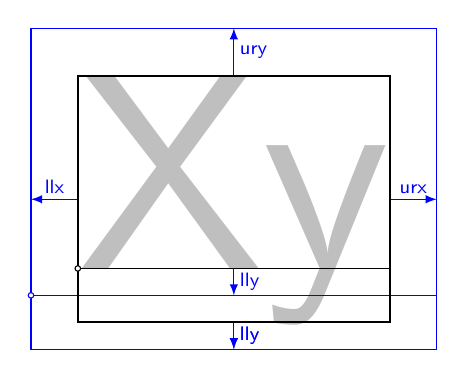
\begin{tikzpicture}[font=\sffamily,>=latex]
% Save example text in box
   \def\text{\scalebox{10}{Xy}}
   \sbox\mybox{\pgfinterruptpicture\sffamily\color{black!25}\scalebox{10}{Xy}\endpgfinterruptpicture}
   \def\HEIGHT{\ht\mybox}
   \def\WIDTH{\wd\mybox}
   \def\DEPTH{\dp\mybox}
   \def\LLX{.15\WIDTH}
   \def\LLY{.5\DEPTH}
   \def\URX{.15\WIDTH}
   \def\URY{.25\HEIGHT}
% Text node:
   \node [inner sep=0pt,anchor=base west] {\usebox\mybox};
% Baseline
   \draw (0,0) -- (\WIDTH,0);% node [above,midway] {baseline};
%\draw [<-,shorten <=2pt] (0,0) -- (2ex,-2ex) -- +(.5ex,0) node [right=-0.5ex] {origin};
% Dimensions
   \begin{scope}[blue,every node/.append style={inner sep=2pt}]
    \begin{scope}
        \draw ([shift={(-\LLX,-\LLY)}]0,-\DEPTH) rectangle ([shift={(\URX,\URY)}]\WIDTH,\HEIGHT);
%\node [inner sep=0pt,anchor=base west,color=blue!50!white] {\text};
    \end{scope}
%\draw [->,.!45] (\WIDTH,\HEIGHT) -- ++(-\URX,-\URY);
%\draw [->,.!45] (0,-\DEPTH) -- ++(\LLX,\LLY);
    \draw [->] (.5\WIDTH,-\DEPTH) -- ++(0,-\LLY) node [right,midway] {\scriptsize lly};
    \draw [->] (0,.5*\HEIGHT-.5*\DEPTH) -- ++(-\LLX,0) node [above,midway] {\scriptsize llx};
    \draw [->] (.5\WIDTH,\HEIGHT) -- ++(0,\URY) node [right,midway] {\scriptsize ury};
    \draw [->] (\WIDTH,.5*\HEIGHT-.5*\DEPTH) -- ++(\URX,0) node [above,midway] {\scriptsize urx};
    \draw [->] (.5\WIDTH,-\DEPTH) -- ++(0,-\LLY) node [right,midway] {\scriptsize lly};
    \draw (-\LLX,-\LLY) -- ([shift={(+\URX,0)}]\WIDTH,-\LLY);
    \path [fill=white,draw] (-\LLX,-\LLY) circle (1pt);
    \draw [->] (.5\WIDTH,0pt) -- ++(0,-\LLY) node [right,midway] {\scriptsize lly};
   \end{scope}
% Box
   \draw [thick] (0,-\DEPTH) rectangle (\WIDTH,\HEIGHT);
% Origin
   \path [fill=white,draw=black] (0,0) circle (1pt);
% Center inner box
   \path let
        \p1 = (current bounding box.south west),
        \p2 = (current bounding box.north east),
        \p3 = (0,-\DEPTH),
        \p4 = (\WIDTH,\HEIGHT)
   in
        (\x3-\x2+\x4,\y3) rectangle (\x4+\x3-\x1,\y4);
\end{tikzpicture}
%<*standalone>
\end{document}
%</standalone>
% \iffalse
%</margin2.tex>
% \fi
%
% \iffalse
%<*margin.tex>
% \fi
%<*standalone>
\documentclass{standalone}

\usepackage{tikz}
\usetikzlibrary{calc}
\newsavebox\mybox

\begin{document}
% Diagram of the TeX box model and its dimensions
% Copyright (C) 2001 by Martin Scharrer <martin@scharrer.me>, Nov 12th 2011
% This is free code under the LPPL v1.3 or later version OR the CC BY-SA 3.0
%</standalone>
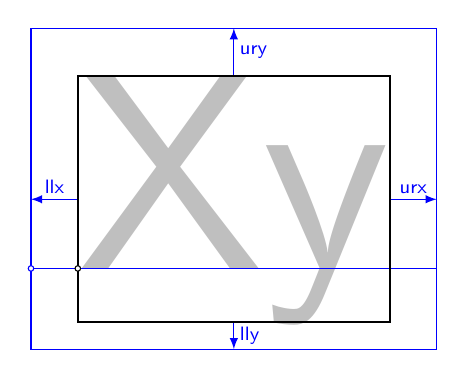
\begin{tikzpicture}[font=\sffamily,>=latex]
% Save example text in box
   \def\text{\scalebox{10}{Xy}}
   \sbox\mybox{\pgfinterruptpicture\sffamily\color{black!25}\scalebox{10}{Xy}\endpgfinterruptpicture}
   \def\HEIGHT{\ht\mybox}
   \def\WIDTH{\wd\mybox}
   \def\DEPTH{\dp\mybox}
   \def\LLX{.15\WIDTH}
   \def\LLY{.5\DEPTH}
   \def\URX{.15\WIDTH}
   \def\URY{.25\HEIGHT}
% Text node:
   \node [inner sep=0pt,anchor=base west] {\usebox\mybox};
% Baseline
   \draw (0,0) -- (\WIDTH,0);% node [above,midway] {baseline};
%\draw [<-,shorten <=2pt] (0,0) -- (2ex,-2ex) -- +(.5ex,0) node [right=-0.5ex] {origin};
% Dimensions
   \begin{scope}[blue,every node/.append style={inner sep=2pt}]
    \begin{scope}
        \draw ([shift={(-\LLX,-\LLY)}]0,-\DEPTH) rectangle ([shift={(\URX,\URY)}]\WIDTH,\HEIGHT);
%\node [inner sep=0pt,anchor=base west,color=blue!50!white] {\text};
    \end{scope}
%\draw [->,.!45] (\WIDTH,\HEIGHT) -- ++(-\URX,-\URY);
%\draw [->,.!45] (0,-\DEPTH) -- ++(\LLX,\LLY);
    \draw [->] (.5\WIDTH,-\DEPTH) -- ++(0,-\LLY) node [right,midway] {\scriptsize lly};
    \draw [->] (0,.5*\HEIGHT-.5*\DEPTH) -- ++(-\LLX,0) node [above,midway] {\scriptsize llx};
    \draw (-\LLX,0) -- ([shift={(+\URX,0)}]\WIDTH,0);
    \draw [->] (.5\WIDTH,\HEIGHT) -- ++(0,\URY) node [right,midway] {\scriptsize ury};
    \draw [->] (\WIDTH,.5*\HEIGHT-.5*\DEPTH) -- ++(\URX,0) node [above,midway] {\scriptsize urx};
    \path [fill=white,draw] (-\LLX,0) circle (1pt);
   \end{scope}
% Box
   \draw [thick] (0,-\DEPTH) rectangle (\WIDTH,\HEIGHT);
% Origin
   \path [fill=white,draw=black] (0,0) circle (1pt);
% Center inner box
   \path let
        \p1 = (current bounding box.south west),
        \p2 = (current bounding box.north east),
        \p3 = (0,-\DEPTH),
        \p4 = (\WIDTH,\HEIGHT)
   in
        (\x3-\x2+\x4,\y3) rectangle (\x4+\x3-\x1,\y4);
\end{tikzpicture}
%<*standalone>
\end{document}
%</standalone>
% \iffalse
%</margin.tex>
% \fi
%
% \iffalse
%<*trim2.tex>
% \fi
%<*standalone>
\documentclass{standalone}

\usepackage{tikz}
\usetikzlibrary{calc}
\usepackage{adjustbox}
\newsavebox\mybox

\begin{document}
%</standalone>
% Diagram of the TeX box model and its dimensions
% Copyright (C) 2001 by Martin Scharrer <martin@scharrer.me>, Nov 12th 2011
% This is free code under the LPPL v1.3 or later version OR the CC BY-SA 3.0

% Save example text in box
\def\text{\sffamily\scalebox{10}{Xy}}
\sbox\mybox{\sffamily\color{black!25}\scalebox{10}{Xy}}
\def\HEIGHT{\ht\mybox}
\def\WIDTH{\wd\mybox}
\def\DEPTH{\dp\mybox}
\def\LLX{.15\WIDTH}
\def\LLY{\DEPTH+.15\HEIGHT}
\def\URX{.15\WIDTH}
\def\URY{.25\HEIGHT}
%
%\usebox\mybox
%\rlap{\trimbox{{\LLX} {\LLY} {\URX} {\URY}}{\usebox\mybox}}\clipbox{{\LLX} {\LLY} {\URX} {\URY}}{\color{blue}{\text}}
\begin{tikzpicture}[font=\sffamily,>=latex]
% Extensions lines for dimensions (drawn here to be below other material)
   \draw [gray,thin]
        (0,0)       -- +(-3.5ex,0)
        (0,\HEIGHT) -- +(-3.5ex,0)
        (0,-\DEPTH) -- +(-3.5ex,0)
        (\WIDTH,\HEIGHT) -- +(3.5ex,0)
        (\WIDTH,-\DEPTH) -- +(3.5ex,0)
        (0,-\DEPTH)      -- +(0,-3.5ex)
        (\WIDTH,-\DEPTH) -- +(0,-3.5ex)
   ;
% Text node:
   \node [inner sep=0pt,anchor=base west] {\usebox\mybox};
% Baseline
   \draw (0,0) -- (\WIDTH,0);% node [above,midway] {baseline};
%\draw [<-,shorten <=2pt] (0,0) -- (2ex,-2ex) -- +(.5ex,0) node [right=-0.5ex] {origin};
% Dimensions
   \draw [->] (-2.5ex,0) -- +(0,-\DEPTH)  node [midway,left] {depth};
   \draw [->] (-2.5ex,0) -- +(0, \HEIGHT) node [midway,left] {height};
   \draw [<->] (\WIDTH,-\DEPTH) ++(2.5ex,0) -- +(0,\DEPTH+\HEIGHT) node [midway,right] {totalheight};
   \draw [<->] (0,-\DEPTH) ++(0,-2.5ex) -- +(\WIDTH,0) node [midway,below] {width};
   \fill (-2.5ex,0) circle (.5pt);
   \begin{scope}[blue] %,every node/.append style={inner sep=2pt}]
    \begin{scope}
        \clip ([shift={(\LLX,\LLY)}]0,-\DEPTH) rectangle ([shift={(-\URX,-\URY)}]\WIDTH,\HEIGHT);
        \node [inner sep=0pt,anchor=base west,color=blue!50!white] {\text};
    \end{scope}
%\draw [->,.!45] (\WIDTH,\HEIGHT) -- ++(-\URX,-\URY);
%\draw [->,.!45] (0,-\DEPTH) -- ++(\LLX,\LLY);
    \draw ([shift={(\LLX,\LLY)}]0,-\DEPTH) rectangle ([shift={(-\URX,-\URY)}]\WIDTH,\HEIGHT);
    \draw [->] (\LLX,-\DEPTH)   -- ++(0,\LLY) node [right,midway] {\scriptsize lly};
    \draw [->] (0,-\DEPTH+\LLY) -- ++(\LLX,0) node [above,midway] {\scriptsize llx};
    \draw (\LLX,-\DEPTH+\LLY) -- ([shift={(-\URX,0)}]\WIDTH,-\DEPTH+\LLY);
    \draw [->] (\LLX+.2\WIDTH,-\DEPTH+\LLY) -- (\LLX+.2\WIDTH,0) node [right,midway] {\scriptsize moves down};
    \path [fill=white,draw] (\LLX,-\DEPTH+\LLY) circle (1pt);
    \draw [->]
        ([shift={(-\URX,0)}]\WIDTH,\HEIGHT) --
        ([shift={(-\URX,-\URY)}]\WIDTH,\HEIGHT)
        node [left,midway] {\scriptsize ury}
    ;
    \draw [->]
        ([shift={(0,-\URY)}]\WIDTH,\HEIGHT) --
        ([shift={(-\URX,-\URY)}]\WIDTH,\HEIGHT)
        node [below,midway] {\scriptsize urx}
    ;
   \end{scope}
% Box
   \draw [thick] (0,-\DEPTH) rectangle (\WIDTH,\HEIGHT);
% Origin
   \path [fill=white,draw=black] (0,0) circle (1pt);
% Center inner box
   \path let
        \p1 = (current bounding box.south west),
        \p2 = (current bounding box.north east),
        \p3 = (0,-\DEPTH),
        \p4 = (\WIDTH,\HEIGHT)
   in
        (\x3-\x2+\x4,\y3) rectangle (\x4+\x3-\x1,\y4);
\end{tikzpicture}
%<*standalone>
\end{document}
%</standalone>
% \iffalse
%</trim2.tex>
% \fi
%
% \iffalse
%<*trim3.tex>
% \fi
%<*standalone>
\documentclass{standalone}

\usepackage{tikz}
\usetikzlibrary{calc}
\usepackage{adjustbox}
\newsavebox\mybox

\begin{document}
%</standalone>
% Diagram of the TeX box model and its dimensions
% Copyright (C) 2001 by Martin Scharrer <martin@scharrer.me>, Nov 12th 2011
% This is free code under the LPPL v1.3 or later version OR the CC BY-SA 3.0

% Save example text in box
\def\text{\sffamily\scalebox{10}{Xy}}
\sbox\mybox{\sffamily\color{black!25}\scalebox{10}{Xy}}
\def\HEIGHT{\ht\mybox}
\def\WIDTH{\wd\mybox}
\def\DEPTH{\dp\mybox}
\def\LLX{.15\WIDTH}
\def\LLY{.4\DEPTH}
\def\URX{.15\WIDTH}
\def\URY{(\HEIGHT+.25\DEPTH)}
%
%\leavevmode
%\rlap{\hbox to \wd\mybox{\hrulefill}}\usebox\mybox
%\rlap{\hbox to \wd\mybox{\hrulefill}}\rlap{\trimbox{{\LLX} {\LLY} {\URX} {\URY}}{\usebox\mybox}}\clipbox{{\LLX} {\LLY} {\URX} {\URY}}{\color{blue}{\text}}
%\sbox0{\clipbox{{\LLX} {\LLY} {\URX} {\URY}}{\color{blue}{\text}}}%
%ht=\the\ht0, dp=\the\dp0, wd=\the\wd0
\begin{tikzpicture}[font=\sffamily,>=latex]
% Extensions lines for dimensions (drawn here to be below other material)
   \draw [gray,thin]
        (0,0)       -- +(-3.5ex,0)
        (0,\HEIGHT) -- +(-3.5ex,0)
        (0,-\DEPTH) -- +(-3.5ex,0)
        (\WIDTH,\HEIGHT) -- +(3.5ex,0)
        (\WIDTH,-\DEPTH) -- +(3.5ex,0)
        (0,-\DEPTH)      -- +(0,-3.5ex)
        (\WIDTH,-\DEPTH) -- +(0,-3.5ex)
   ;
% Text node:
   \node [inner sep=0pt,anchor=base west] {\usebox\mybox};
% Baseline
   \draw (0,0) -- (\WIDTH,0);% node [above,midway] {baseline};
%\draw [<-,shorten <=2pt] (0,0) -- (2ex,-2ex) -- +(.5ex,0) node [right=-0.5ex] {origin};
% Dimensions
   \draw [->] (-2.5ex,0) -- +(0,-\DEPTH)  node [midway,left] {depth};
   \draw [->] (-2.5ex,0) -- +(0, \HEIGHT) node [midway,left] {height};
   \draw [<->] (\WIDTH,-\DEPTH) ++(2.5ex,0) -- +(0,\DEPTH+\HEIGHT) node [midway,right] {totalheight};
   \draw [<->] (0,-\DEPTH) ++(0,-2.5ex) -- +(\WIDTH,0) node [midway,below] {width};
   \fill (-2.5ex,0) circle (.5pt);
   \begin{scope}[blue] %,every node/.append style={inner sep=2pt}]
    \begin{scope}
        \clip ([shift={(\LLX,\LLY)}]0,-\DEPTH) rectangle ([shift={(-\URX,-\URY)}]\WIDTH,\HEIGHT);
        \node [inner sep=0pt,anchor=base west,color=blue!50!white] {\text};
    \end{scope}
%\draw [->,.!45] (\WIDTH,\HEIGHT) -- ++(-\URX,{-\URY});
%\draw [->,.!45] (0,-\DEPTH)      -- ++(\LLX,\LLY);
    \draw ([shift={(\LLX,\LLY)}]0,-\DEPTH) rectangle ([shift={(-\URX,-\URY)}]\WIDTH,\HEIGHT);
    \draw [->] (\LLX,-\DEPTH)   -- ++(0,\LLY) node [right,midway] {\scriptsize lly};
    \draw [->] (0,-\DEPTH+\LLY) -- ++(\LLX,0) node [above,midway] {\scriptsize llx};
    \draw (\LLX,-\DEPTH+\LLY) -- ([shift={(-\URX,0)}]\WIDTH,-\DEPTH+\LLY);
    \draw [->] (\LLX+.2\WIDTH,{\HEIGHT-\URY}) -- (\LLX+.2\WIDTH,0) node [pos=0.4,below right] {\scriptsize moves up};
    \path [fill=white,draw] (\LLX,{\HEIGHT-\URY}) circle (1pt);
    \draw [->]
        ([shift={(-\URX,0)}]\WIDTH,\HEIGHT) --
        ([shift={(-\URX,-\URY)}]\WIDTH,\HEIGHT)
        node [left,midway] {\scriptsize ury}
    ;
    \draw [->]
        ([shift={(0,-\URY)}]\WIDTH,\HEIGHT) --
        ([shift={(-\URX,-\URY)}]\WIDTH,\HEIGHT)
        node [below,midway] {\scriptsize urx}
    ;
   \end{scope}
% Box
   \draw [thick] (0,-\DEPTH) rectangle (\WIDTH,\HEIGHT);
% Origin
   \path [fill=white,draw=black] (0,0) circle (1pt);
% Center inner box
   \path let
        \p1 = (current bounding box.south west),
        \p2 = (current bounding box.north east),
        \p3 = (0,-\DEPTH),
        \p4 = (\WIDTH,\HEIGHT)
   in
        (\x3-\x2+\x4,\y3) rectangle (\x4+\x3-\x1,\y4);
\end{tikzpicture}
%<*standalone>
\end{document}
%</standalone>
% \iffalse
%</trim3.tex>
% \fi
%
% \iffalse
%<*trim.tex>
% \fi
%<*standalone>
\documentclass{standalone}

\usepackage{tikz}
\usetikzlibrary{calc}
\newsavebox\mybox

\begin{document}
%</standalone>
% Diagram of the TeX box model and its dimensions
% Copyright (C) 2001 by Martin Scharrer <martin@scharrer.me>, Nov 12th 2011
% This is free code under the LPPL v1.3 or later version OR the CC BY-SA 3.0
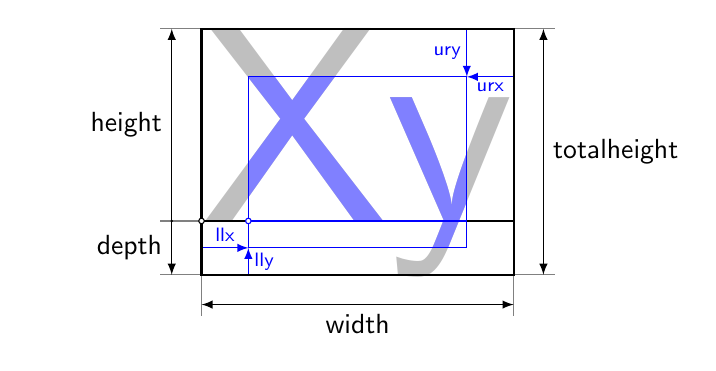
\begin{tikzpicture}[font=\sffamily,>=latex]
% Save example text in box
   \def\text{\scalebox{10}{Xy}}
   \sbox\mybox{\pgfinterruptpicture\sffamily\color{black!25}\scalebox{10}{Xy}\endpgfinterruptpicture}
   \def\HEIGHT{\ht\mybox}
   \def\WIDTH{\wd\mybox}
   \def\DEPTH{\dp\mybox}
   \def\LLX{.15\WIDTH}
   \def\LLY{.5\DEPTH}
   \def\URX{.15\WIDTH}
   \def\URY{.25\HEIGHT}
% Extensions lines for dimensions (drawn here to be below other material)
   \draw [gray,thin]
        (0,0)       -- +(-3.5ex,0)
        (0,\HEIGHT) -- +(-3.5ex,0)
        (0,-\DEPTH) -- +(-3.5ex,0)
        (\WIDTH,\HEIGHT) -- +(3.5ex,0)
        (\WIDTH,-\DEPTH) -- +(3.5ex,0)
        (0,-\DEPTH)      -- +(0,-3.5ex)
        (\WIDTH,-\DEPTH) -- +(0,-3.5ex)
   ;
% Text node:
   \node [inner sep=0pt,anchor=base west] {\usebox\mybox};
% Baseline
   \draw (0,0) -- (\WIDTH,0);% node [above,midway] {baseline};
%\draw [<-,shorten <=2pt] (0,0) -- (2ex,-2ex) -- +(.5ex,0) node [right=-0.5ex] {origin};
% Dimensions
   \draw [->] (-2.5ex,0) -- +(0,-\DEPTH)  node [midway,left] {depth};
   \draw [->] (-2.5ex,0) -- +(0, \HEIGHT) node [midway,left] {height};
   \draw [<->] (\WIDTH,-\DEPTH) ++(2.5ex,0) -- +(0,\DEPTH+\HEIGHT) node [midway,right] {totalheight};
   \draw [<->] (0,-\DEPTH) ++(0,-2.5ex) -- +(\WIDTH,0) node [midway,below] {width};
   \fill (-2.5ex,0) circle (.5pt);
   \begin{scope}[blue,every node/.append style={inner sep=2pt}]
    \begin{scope}
        \clip ([shift={(\LLX,\LLY)}]0,-\DEPTH) rectangle ([shift={(-\URX,-\URY)}]\WIDTH,\HEIGHT);
        \node [inner sep=0pt,anchor=base west,color=blue!50!white] {\text};
    \end{scope}
%\draw [->,.!45] (\WIDTH,\HEIGHT) -- ++(-\URX,-\URY);
%\draw [->,.!45] (0,-\DEPTH) -- ++(\LLX,\LLY);
    \draw ([shift={(\LLX,\LLY)}]0,-\DEPTH) rectangle ([shift={(-\URX,-\URY)}]\WIDTH,\HEIGHT);
    \draw [->] (\LLX,-\DEPTH)   -- ++(0,\LLY) node [right,midway] {\scriptsize lly};
    \draw [->] (0,-\DEPTH+\LLY) -- ++(\LLX,0) node [above,midway] {\scriptsize llx};
    \draw (\LLX,0) -- ([shift={(-\URX,0)}]\WIDTH,0);
    \draw [->]
        ([shift={(-\URX,0)}]\WIDTH,\HEIGHT) --
        ([shift={(-\URX,-\URY)}]\WIDTH,\HEIGHT)
        node [left,midway] {\scriptsize ury}
    ;
    \draw [->]
        ([shift={(0,-\URY)}]\WIDTH,\HEIGHT) --
        ([shift={(-\URX,-\URY)}]\WIDTH,\HEIGHT)
        node [below,midway] {\scriptsize urx}
    ;
    \path [fill=white,draw] (\LLX,0) circle (1pt);
   \end{scope}
% Box
   \draw [thick] (0,-\DEPTH) rectangle (\WIDTH,\HEIGHT);
% Origin
   \path [fill=white,draw=black] (0,0) circle (1pt);
% Center inner box
   \path let
        \p1 = (current bounding box.south west),
        \p2 = (current bounding box.north east),
        \p3 = (0,-\DEPTH),
        \p4 = (\WIDTH,\HEIGHT)
   in
        (\x3-\x2+\x4,\y3) rectangle (\x4+\x3-\x1,\y4);
\end{tikzpicture}
%<*standalone>
\end{document}
%</standalone>
% \iffalse
%</trim.tex>
% \fi
%
% \iffalse
%<*viewport2.tex>
% \fi
%<*standalone>
\documentclass{standalone}

\usepackage{tikz}
\usetikzlibrary{calc}
\usepackage{adjustbox}
\newsavebox\mybox

\begin{document}
%</standalone>
% Diagram of the TeX box model and its dimensions
% Copyright (C) 2001 by Martin Scharrer <martin@scharrer.me>, Nov 12th 2011
% This is free code under the LPPL v1.3 or later version OR the CC BY-SA 3.0

% Save example text in box
\def\text{\sffamily\scalebox{10}{Xy}}
\sbox\mybox{\sffamily\color{black!25}\scalebox{10}{Xy}}
\def\HEIGHT{\ht\mybox}
\def\WIDTH{\wd\mybox}
\def\DEPTH{\dp\mybox}
\def\LLX{.15\WIDTH}
\def\LLY{\DEPTH-.15\HEIGHT}
\def\URX{.15\WIDTH}
\def\URY{.25\HEIGHT}
%
%\usebox\mybox
%\rlap{\trimbox{{\LLX} {\LLY} {\URX} {\URY}}{\usebox\mybox}}\clipbox{{\LLX} {\LLY} {\URX} {\URY}}{\color{blue}{\text}}
\begin{tikzpicture}[font=\sffamily,>=latex]
% Extensions lines for dimensions (drawn here to be below other material)
   \draw [gray,thin]
        (0,0)       -- +(-3.5ex,0)
        (0,\HEIGHT) -- +(-3.5ex,0)
        (0,-\DEPTH) -- +(-3.5ex,0)
        (\WIDTH,\HEIGHT) -- +(3.5ex,0)
        (\WIDTH,-\DEPTH) -- +(3.5ex,0)
        (0,-\DEPTH)      -- +(0,-3.5ex)
        (\WIDTH,-\DEPTH) -- +(0,-3.5ex)
   ;
% Text node:
   \node [inner sep=0pt,anchor=base west] {\usebox\mybox};
% Baseline
   \draw (0,0) -- (\WIDTH,0);% node [above,midway] {baseline};
%\draw [<-,shorten <=2pt] (0,0) -- (2ex,-2ex) -- +(.5ex,0) node [right=-0.5ex] {origin};
% Dimensions
   \draw [->] (-2.5ex,0) -- +(0,-\DEPTH)  node [midway,left] {depth};
   \draw [->] (-2.5ex,0) -- +(0, \HEIGHT) node [midway,left] {height};
   \draw [<->] (\WIDTH,-\DEPTH) ++(2.5ex,0) -- +(0,\DEPTH+\HEIGHT) node [midway,right] {totalheight};
   \draw [<->] (0,-\DEPTH) ++(0,-2.5ex) -- +(\WIDTH,0) node [midway,below] {width};
   \fill (-2.5ex,0) circle (.5pt);
   \begin{scope}[blue]
        \clip ([shift={(\LLX,\LLY)}]0,-\DEPTH) rectangle ([shift={(-\URX,-\URY)}]\WIDTH,\HEIGHT);
        \node [inner sep=0pt,anchor=base west,color=blue!50!white] {\text};
   \end{scope}
   \begin{scope}[blue]
        \draw ([shift={(\LLX,\LLY)}]0,-\DEPTH) rectangle ([shift={(-\URX,-\URY)}]\WIDTH,\HEIGHT);
        \draw (\LLX,0) -- ([shift={(-\URX,0)}]\WIDTH,0);
        \path [fill=white,draw] (\LLX,0) circle (1pt);
   \end{scope}
   \begin{scope}[blue!50!black] %,every node/.append style={inner sep=2pt}]
%\draw [->,.!45] (0,0) -- ++(-\URX+\WIDTH,-\URY+\HEIGHT);
%\draw [->,.!45] (0,0) -- ++(\LLX,\LLY-\DEPTH);
    \draw [->] (\LLX,0) -- (\LLX,\LLY-\DEPTH) node [right,midway] {\scriptsize lly};
    \draw [->] (0,-\DEPTH+\LLY) -- ++(\LLX,0) node [above,midway] {\scriptsize llx};
    \draw [->]
        ([shift={(-\URX,0)}]\WIDTH,0) --
        ([shift={(-\URX,-\URY)}]\WIDTH,\HEIGHT)
        node [right,midway] {\scriptsize ury}
    ;
    \draw [->]
        ([shift={(0,-\URY)}]0,\HEIGHT) --
        ([shift={(-\URX,-\URY)}]\WIDTH,\HEIGHT)
        node [above,midway] {\scriptsize urx}
    ;
   \end{scope}
% Box
   \draw [thick] (0,-\DEPTH) rectangle (\WIDTH,\HEIGHT);
% Origin
   \path [fill=white,draw=black] (0,0) circle (1pt);
% Center inner box
   \path let
        \p1 = (current bounding box.south west),
        \p2 = (current bounding box.north east),
        \p3 = (0,-\DEPTH),
        \p4 = (\WIDTH,\HEIGHT)
   in
        (\x3-\x2+\x4,\y3) rectangle (\x4+\x3-\x1,\y4);
\end{tikzpicture}
%<*standalone>
\end{document}
%</standalone>
% \iffalse
%</viewport2.tex>
% \fi
%
% \iffalse
%<*viewport.tex>
% \fi
%<*standalone>
\documentclass{standalone}

\usepackage{tikz}
\usetikzlibrary{calc}
\usepackage{adjustbox}
\newsavebox\mybox

\begin{document}
%</standalone>
% Diagram of the TeX box model and its dimensions
% Copyright (C) 2001 by Martin Scharrer <martin@scharrer.me>, Nov 12th 2011
% This is free code under the LPPL v1.3 or later version OR the CC BY-SA 3.0

% Save example text in box
\def\text{\sffamily\scalebox{10}{Xy}}
\sbox\mybox{\sffamily\color{black!25}\scalebox{10}{Xy}}
\def\HEIGHT{\ht\mybox}
\def\WIDTH{\wd\mybox}
\def\DEPTH{\dp\mybox}
\def\LLX{.15\WIDTH}
\def\LLY{\DEPTH+.15\HEIGHT}
\def\URX{.15\WIDTH}
\def\URY{.25\HEIGHT}
%
%\usebox\mybox
%\rlap{\trimbox{{\LLX} {\LLY} {\URX} {\URY}}{\usebox\mybox}}\clipbox{{\LLX} {\LLY} {\URX} {\URY}}{\color{blue}{\text}}
\begin{tikzpicture}[font=\sffamily,>=latex]
% Extensions lines for dimensions (drawn here to be below other material)
   \draw [gray,thin]
        (0,0)       -- +(-3.5ex,0)
        (0,\HEIGHT) -- +(-3.5ex,0)
        (0,-\DEPTH) -- +(-3.5ex,0)
        (\WIDTH,\HEIGHT) -- +(3.5ex,0)
        (\WIDTH,-\DEPTH) -- +(3.5ex,0)
        (0,-\DEPTH)      -- +(0,-3.5ex)
        (\WIDTH,-\DEPTH) -- +(0,-3.5ex)
   ;
% Text node:
   \node [inner sep=0pt,anchor=base west] {\usebox\mybox};
% Baseline
   \draw (0,0) -- (\WIDTH,0);% node [above,midway] {baseline};
%\draw [<-,shorten <=2pt] (0,0) -- (2ex,-2ex) -- +(.5ex,0) node [right=-0.5ex] {origin};
% Dimensions
   \draw [->] (-2.5ex,0) -- +(0,-\DEPTH)  node [midway,left] {depth};
   \draw [->] (-2.5ex,0) -- +(0, \HEIGHT) node [midway,left] {height};
   \draw [<->] (\WIDTH,-\DEPTH) ++(2.5ex,0) -- +(0,\DEPTH+\HEIGHT) node [midway,right] {totalheight};
   \draw [<->] (0,-\DEPTH) ++(0,-2.5ex) -- +(\WIDTH,0) node [midway,below] {width};
   \fill (-2.5ex,0) circle (.5pt);
   \begin{scope}[blue]
        \clip ([shift={(\LLX,\LLY)}]0,-\DEPTH) rectangle ([shift={(-\URX,-\URY)}]\WIDTH,\HEIGHT);
        \node [inner sep=0pt,anchor=base west,color=blue!50!white] {\text};
   \end{scope}
   \begin{scope}[blue]
%\draw [->,.!45] (0,0) -- ++(-\URX+\WIDTH,-\URY+\HEIGHT);
%\draw [->,.!45] (0,0) -- ++(\LLX,\LLY-\DEPTH);
        \draw ([shift={(\LLX,\LLY)}]0,-\DEPTH) rectangle ([shift={(-\URX,-\URY)}]\WIDTH,\HEIGHT);
        \draw (\LLX,-\DEPTH+\LLY) -- ([shift={(-\URX,0)}]\WIDTH,-\DEPTH+\LLY);
        \draw [->] (\LLX+.2\WIDTH,-\DEPTH+\LLY) -- (\LLX+.2\WIDTH,0) node [right,midway] {\scriptsize moves down};
        \path [fill=white,draw] (\LLX,-\DEPTH+\LLY) circle (1pt);
   \end{scope}
   \begin{scope}[blue!50!black] %,every node/.append style={inner sep=2pt}]
    \draw [->] (\LLX,0) -- (\LLX,\LLY-\DEPTH) node [right,midway] {\scriptsize lly};
    \draw [->] (0,-\DEPTH+\LLY) -- ++(\LLX,0) node [above,midway] {\scriptsize llx};
    \draw [->]
        ([shift={(-\URX,0)}]\WIDTH,0) --
        ([shift={(-\URX,-\URY)}]\WIDTH,\HEIGHT)
        node [right,midway] {\scriptsize ury}
    ;
    \draw [->]
        ([shift={(0,-\URY)}]0,\HEIGHT) --
        ([shift={(-\URX,-\URY)}]\WIDTH,\HEIGHT)
        node [above,midway] {\scriptsize urx}
    ;
   \end{scope}
% Box
   \draw [thick] (0,-\DEPTH) rectangle (\WIDTH,\HEIGHT);
% Origin
   \path [fill=white,draw=black] (0,0) circle (1pt);
% Center inner box
   \path let
        \p1 = (current bounding box.south west),
        \p2 = (current bounding box.north east),
        \p3 = (0,-\DEPTH),
        \p4 = (\WIDTH,\HEIGHT)
   in
        (\x3-\x2+\x4,\y3) rectangle (\x4+\x3-\x1,\y4);
\end{tikzpicture}
%<*standalone>
\end{document}
%</standalone>
% \iffalse
%</viewport.tex>
% \fi
%